\documentclass[master=ebin,english]{kulemt}
\setup{title={Global-To-Local Segmentation and Genotypic Analysis Of Brain Shape Asymmetry},author={Vasileios Lemonidis},promoter={Prof. Peter Claes \and Prof. Isabelle Cleynen}, assessor=,assistant={MSc. Meng Yuan \and MSc. Seppe Goovaerts},acyear=2022,bind=3mm,inputenc=utf8}
\setup{font=lm}

\usepackage{float}
\usepackage{svg}
\usepackage[pdfusetitle,hidelinks,plainpages=false]{hyperref}

\usepackage{subcaption}
\usepackage[numbers]{natbib}
\bibliographystyle{plainnat}
\graphicspath{
	{../results},
	 {graphics}
}
\usepackage{acro}
\acsetup{
	make-links = true , % boolean
	list/display=all,
	subsequent-style =short
	}
\DeclareAcronym{gwas}{
short=GWAS,
long=genome-wide association studies
}
\DeclareAcronym{mvgwas}{
short=mvGWAS,
short-plural-form=mvGWAS,
long=multivariate genome-wide association study,
long-plural-form=multivariate genome-wide association studies}
\DeclareAcronym{da}{
	short=DA,
	long=directional asymmetry
}
\DeclareAcronym{mri}{
short=MRI,
long=magnetic resonance imaging
}

\DeclareAcronym{snp}{
	short=SNP,
	long=single nucleotide polymorphism}
\DeclareAcronym{hsc}{
	short=HSC,
	long=hierarchical spectral clustering}
\DeclareAcronym{cca}{
	short=CCA,
	long=canonical correlation analysis}
\DeclareAcronym{ld}{
	short=LD,
	long=linkage disequilibrium}
\DeclareAcronym{fa}{
	short=FA,
	long=fluctuating asymmetry}
\DeclareAcronym{anova}{
short=ANOVA,
long=analysis of variance}
\DeclareAcronym{rss}{
short=RSS,
long=residual sum of squares}
\DeclareAcronym{dof}{
short=DOF,
long=degree of freedom,
short-plural=s,
long-plural-form=degrees of freedom}
\DeclareAcronym{dna}{
	short=DNA,
long=deoxyribonucleic acid}
\DeclareAcronym{rna}{
	short=RNA,
	long=ribonucleic acid}

\DeclareAcronym{cns}{
short=CNS,
long=central neural system
}
\DeclareAcronym{rc}{
short=R-C,
long=rostral-caudal}
\DeclareAcronym{dv}{
short=D-V,
long=dorsal-ventral}
\DeclareAcronym{lr}{
	short=L-R,
long=left-right}
\DeclareAcronym{rgc}{
short=RGC,
long=radial glial cell,
short-plural=s,
long-plural=s
}
\DeclareAcronym{npc}{
short=NPC,
long=neuroepithelial cell,
short-plural=s,
long-plural=s}
\DeclareAcronym{3d}{
short=3D,
long=three-dimensional}
\DeclareAcronym{dk}{short=DK,long=Desikan-Killiany}
\DeclareAcronym{adhd}{short=ADHD,long=attention-deficit / hyperactivity-disorder}
\DeclareAcronym{gpa}{short=GPA, long=generalized Procrustes analysis}
\DeclareAcronym{maf}{short=MAF, long=minor allele frequency}
\DeclareAcronym{tf}{short=TF, long=transcription factor}
\DeclareAcronym{glm}{short=GLM, long=generalized linear model}
\DeclareAcronym{fdr}{short=FDR, long=false discovery rate}
\DeclareAcronym{ml}{short=ML, long=machine learning}
\DeclareAcronym{ldsr}{short=LDSR, long=LD score regression}
\DeclareAcronym{ldsc}{short=LDSC, long=LD score correlation}
\DeclareAcronym{gsea}{short=GSEA, long=gene set enrichment analysis}
\DeclareAcronym{grm}{short=GRM, long=genetic relationship matrix}
\DeclareAcronym{go}{short=GO, long=gene ontology}
\DeclareAcronym{ai}{
	short=AI, 
	long =asymmetry index,
	long-plural-form=asymmetry indices}
\DeclareAcronym{asd}{short=ASD, long =autism spectrum disorder }
\DeclareAcronym{ad}{short =AD , long=Alzheimer's disease}
\DeclareAcronym{pd}{short =PD , long=Parkinson's disease}

\DeclareAcronym{hcp}{short=HCP , long=Human Connectome Project}
\DeclareAcronym{pca}{short=PCA, long=principal component analysis}
\DeclareAcronym{plsr}{short=PLSR, long=partial least squares regression}
\DeclareAcronym{pc}{short=PC, long=principal component}
\DeclareAcronym{bd}{short=BD, long=bipolar disorder}
\DeclareAcronym{mdd}{short=MDD, long=major depressive disorder}
\DeclareAcronym{lfc}{short=LFC, long=language functional connectivity}
\DeclareAcronym{ocd}{short=OCD, long=obsessive/compulsive disorder}
\DeclareAcronym{mss}{short=MSS, long=mean sum of squares}
\DeclareAcronym{nmi}{short=NMI, long=normalized mutual information}
\DeclareAcronym{ldsc-seg}{short=LDSC-SEG, long=LD score regression applied to specifically expressed genes}
\DeclareAcronym{svd}{short=SVD, long=singular value decomposition}
\makeatletter\AtBeginDocument{\let\@elt\relax}\makeatother

\begin{document}
	\begin{preface}[The Author\\ \textup{1 January 2010}]
		The text of the preface. A few paragraphs should follow.
	\end{preface}
\tableofcontents*
\cleardoublepage
\listoffigures
\listoftables
\cleardoublepage
\addcontentsline{toc}{chapter}{List of Abbreviations}
\printacronyms[name=Abbreviations]
\begin{abstract}
	Overall purpose of this thesis is to complement the existing bibliography on the detection and examination of the genetic associations of brain shape asymmetry. Asymmetry components  are computed based on the  brain \ac{mri} dataset provided by UK Biobank database. A data-driven approach is followed, where the brain surface is partitioned in an unsupervised manner, through  \ac{hsc}, a technique that allows for  a coarse-to-fine segmentation. Aggregated asymmetry measurements are retrieved from the segments, whose genetic correlation is examined through a \ac{mvgwas} statistical analysis. Recognized significant \acp{snp} are then analyzed individually or in groups, through comparison with existing results and databases.  The genetic overlap with neurodevelopmental disorders and traits, that have been reported to exhibit phenotypic associations with brain structure asymmetry, such as autism, Alzheimer’s disease or intelligence, are examined. Functional annotations of variants associated with the genes where significant \acp{snp} were detected are constructed, offering an insight into the functional reasoning behind the brain shape asymmetry existence.
\end{abstract}
\acresetall
\mainmatter
\chapter{Introduction}
\label{chap:introduction}
\section{Biomedical and anatomic principles}
\subsection{Bilateria lineage}
Cerebral bilateral symmetry is a universal quality of organisms belonging to the Bilateria lineage \cite{Concha2012,Corballis2009}, the phylum incorporating all species with a single plane of symmetry, in contrast with their sister group, Cnidaria (\autoref{fig:bilateriaphylum}). Bilateral symmetry is a byproduct of the activity of two separate developmental processes, that produce two axes of polarity \cite{Finnerty2003}, and therefore a symmetry plane; the formation of a primary body axis, that corresponds to the long anatomical dimension of the animal, called \acf{rc} (i.e. head-to-tail), primarily dictated by highly conserved controlled activation of HOX genes during cell differentiation; the shaping of a secondary body axis, orthogonal to \ac{rc}, named \acf{dv} (i.e. back-to-front), attributed to a variety of genes,  such as the chromatin organizer CTCF, the left-right determination factor Nodal and central HOX genes \cite{Heger2020}. The remaining axis, \acf{lr}, is the one along which the symmetry pattern is manifested. On account of the high biodiversity that bilateria group includes, only the subgroup of vertebrates is examined in the following literature study. In addition, any reference to symmetry or asymmetry from now on corresponds to the \ac{lr} direction, unless explicitly mentioned.

This study makes an effort to statistically identify the genetic origins of a complex structural phenotype. Hence, examining, based on existing research, the main brain developmental stages is essential to discern the processes that induce bilateral symmetry. An important vertebrates (and bilateria) common characteristic is the germ line \textbf{triploblasticity}: the embryo begins as a flat disk, through a process called \textbf{gastrulation}, with three distinct cell layers; \textbf{endoderm}, \textbf{mesoderm}, and \textbf{ectoderm} \cite{F.Bear2016a}.  Of significance in the neural system formation is the ectoderm, which is initially equivalent to one of the flat disk sides. Under the context of this study, although a fact not directly connected to the brain cortex, it is necessary to mention that the perfect bilateral symmetry pattern appears to break even before gastrulation. In Xenopus (frog species) embryos, during fertilization and the initial 4-cell cleavage of the fertilized egg , the \textbf{cytoskeleton microtubules} appear to asymmetrically localize the ion channels proteins, whose \acs{rna} has been passed on by the mother, with a preference for the right side of the complex \cite{Aw2008}. Chicks embryos also exhibit a similar pattern. The occurrence of asymmetry at this extremely early time point underlines the significant role it has on the embryo development, species fitness, and, concomitantly, the conservation potential of this trait drivers \cite{Aw2009}. Another cellular component that is considered to enhance asymmetry, during gastrulation, is the motile cilia, hair-like organelles on the cell surface with the ability to beat \cite{Grimes2017}. Their movement is by construction asymmetric, causing a leftward flow of extraembryonic fluid and, subsequently, asymmetric distribution of exogenously introduced proteins \cite{Okada2005}. Both studied phenomena point to early initiation of asymmetric genes expression.

\begin{figure}[H]
	\centering
	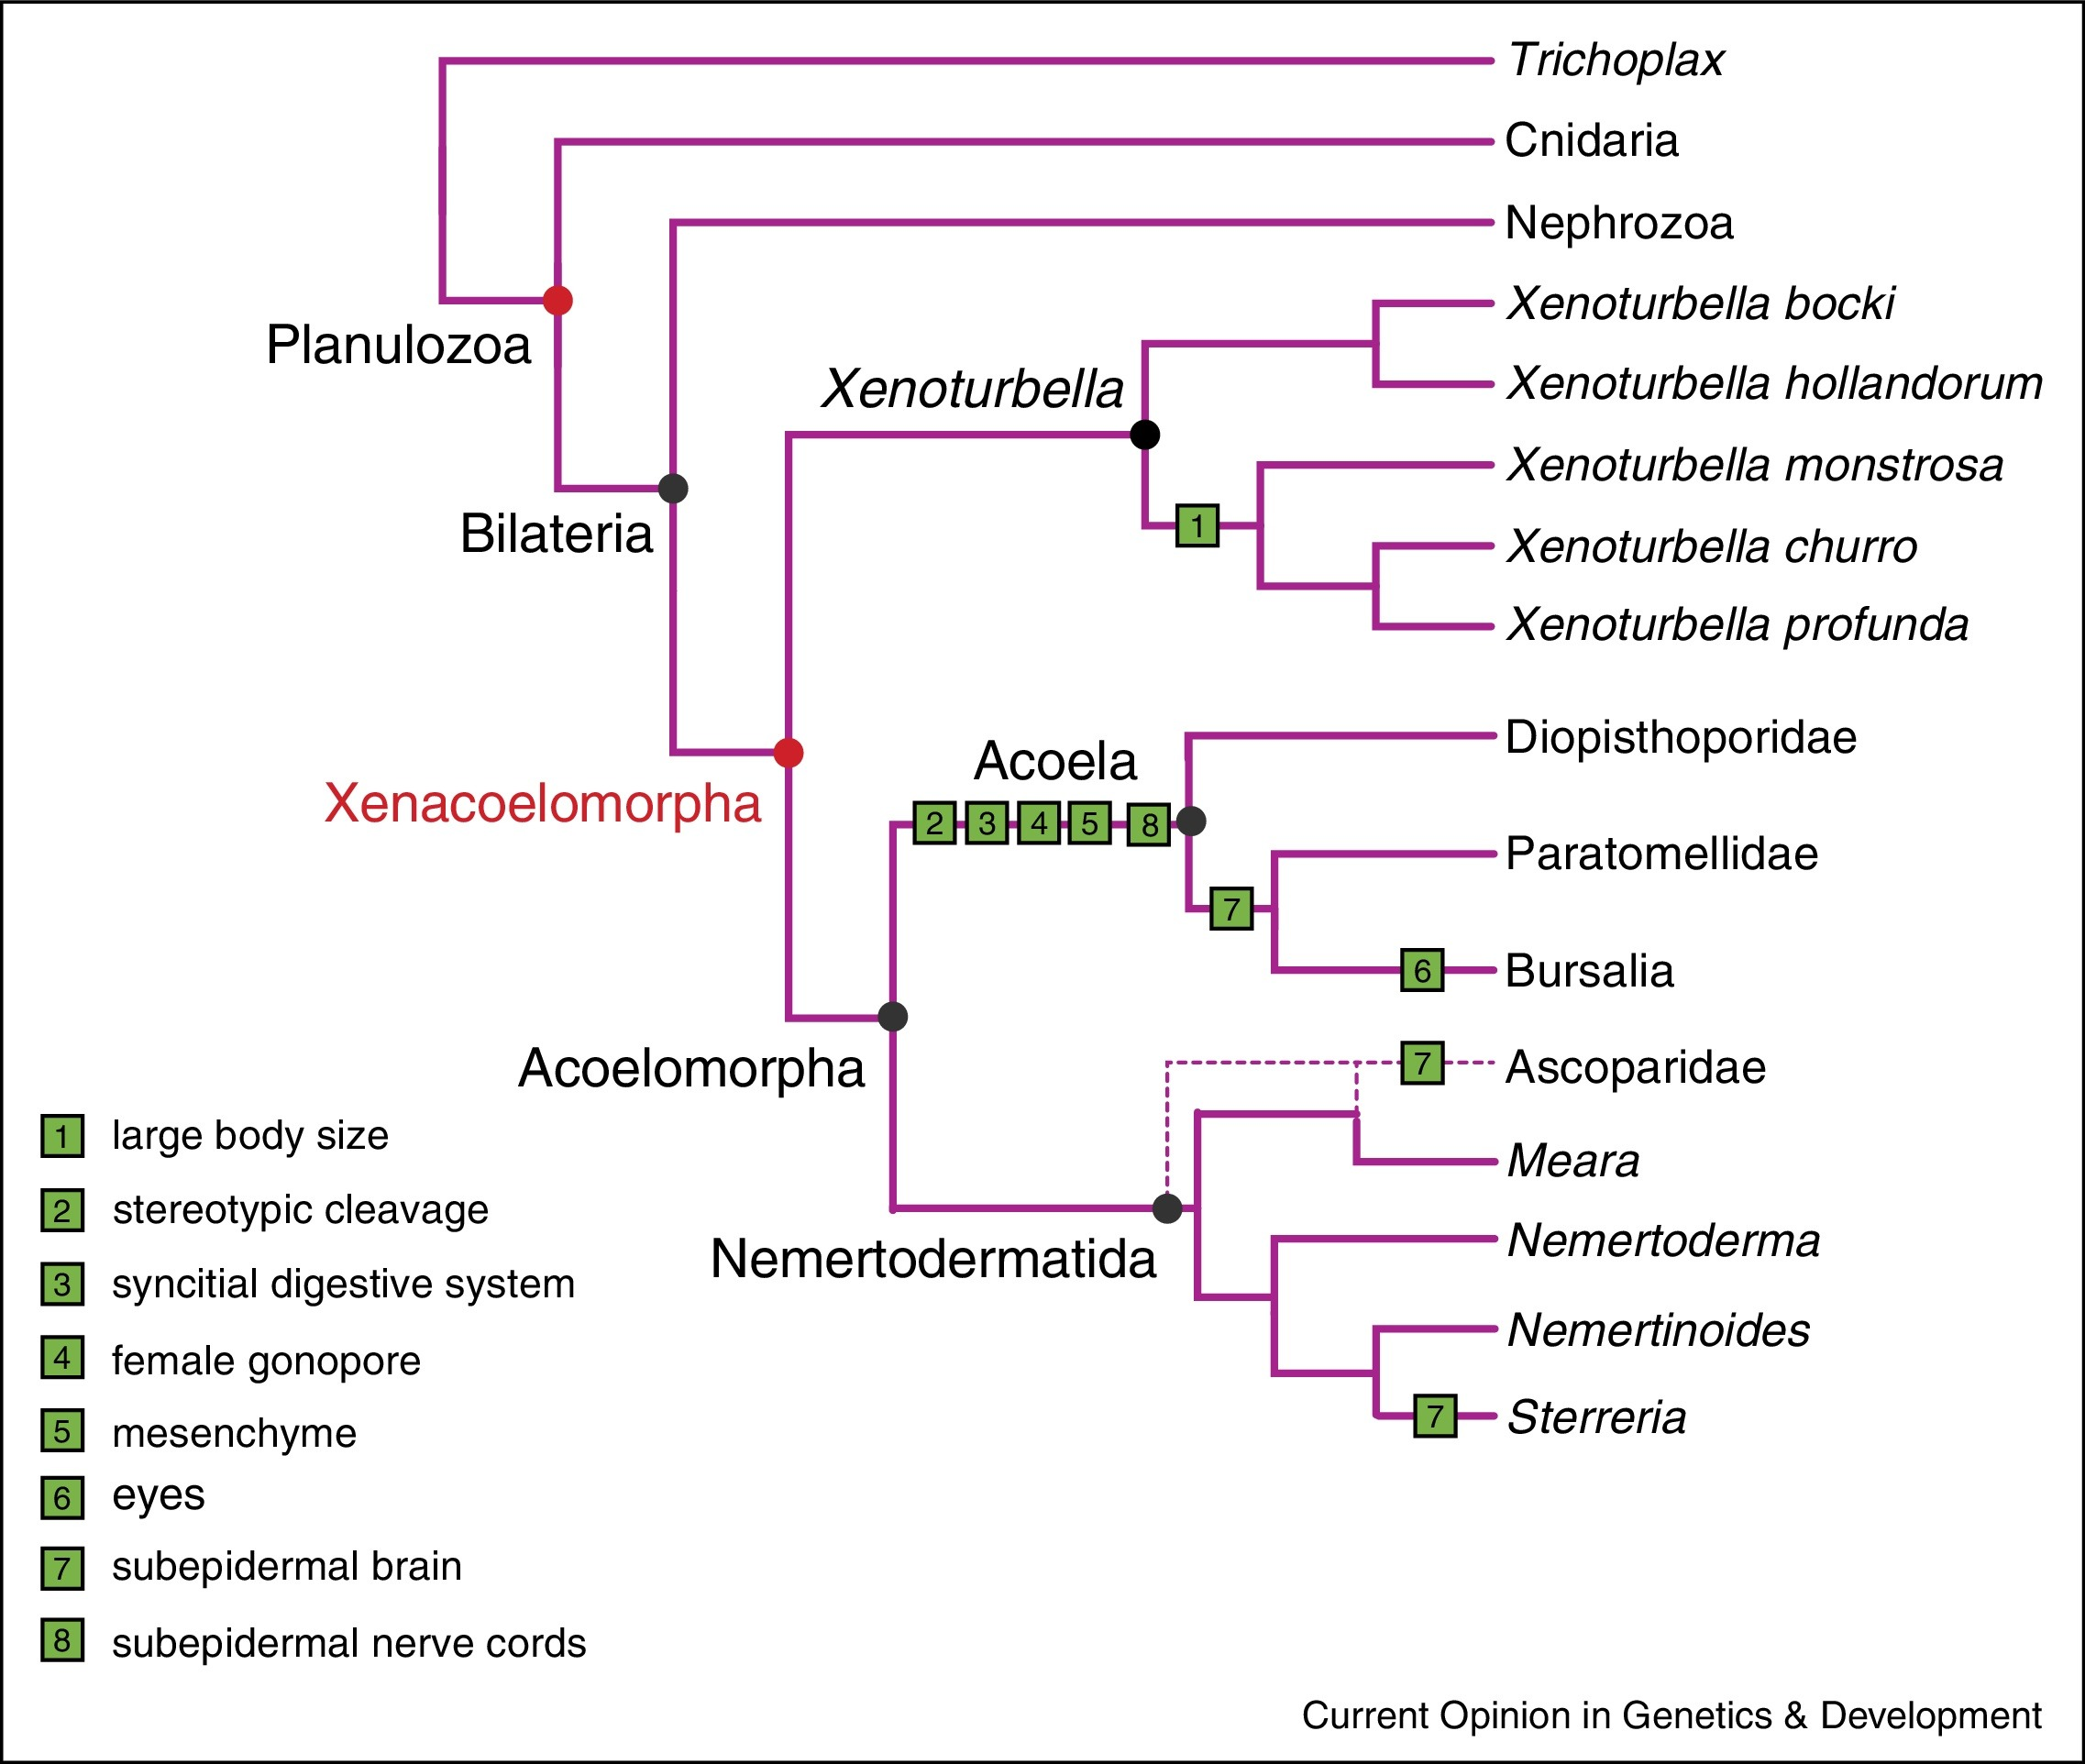
\includegraphics[width=0.9\linewidth]{bilateria_phylum}
	\caption[Bilateria clade \cite{Hejnol2016}]{Species phylogenetic tree subset, displaying bilateria clade, its sister clade, Cnidaria, and the direct children\cite{Hejnol2016}. Of great importance on the evolutionary studies of bilateral symmetry is the Xenacoelomorpha clade.}
	\label{fig:bilateriaphylum}
\end{figure}

\subsection{Symmetry during \acs{cns} formation}
Shortly after gastrulation, the disk folds, in a way that the central region of the ectoderm, called neural plate, forms a tube-like shape, the \textbf{neural tube}, which acts as the neural system precursor, under a process called \textbf{neurulation}. All bilateria have a \acf{cns}, which entirely develops from the neural tube walls \cite{F.Bear2016a}. The next pivotal step in the brain development, \textbf{differentiation}, leads to the creation of three distinct compartments along \ac{rc} axis, at the neural tube rostral end, the \textbf{prosencephalon} (forebrain), which develops into the brain cerebrum, the \textbf{mesencephalon} (midbrain), and the \textbf{rhombencephalon} (hindbrain), that is later attached to the spinal cord in vertebrates. For the subsequent mechanisms and terminology to be compatible with human cerebrum related literature, the focus is shifted on mammals phylum and, spatially, on the prosencephalon. The differentiation proceeds, with two pairs of lumps extruding symmetrically from the prosencephalon, the \textbf{telencephalic} vesicles, the predecessors of cerebral region, and the optic vesicles, the precursors of optic nerves and retinas, while the central remaining, linking structure is called \textbf{diencephalon} \cite{F.Bear2016b}. The formed symmetry plane is called \textbf{midsagittal}. The telencephalic vesicles continue to grow, expanding also caudally and in parallel with the diencephalon, gradually assuming the form of the two hemispheres, while a new pair of vesicles appears on the rostral part of the diencephalon, giving rise to the \textbf{olfactory bulbs}. The neural tube shape also reacts to the changes, forming four distinct \textbf{ventricles} along the neural tube, with two of them, named \textbf{lateral ventricles}, being mirrored inside each of the telencephalic vesicles. The earliest stage where asymmetry is noted in an anatomic level inside the human brain is during the end of the first trimester of gestation \cite{Abu-Rustum2013}. Specifically, the choroid plexus, a specialized cell network that lies inside the ventricles, attached to the diencephalon, and produces most of the \textbf{cerebrospinal fluid} in the \ac{cns},  develops asymmetrically in each lateral ventricle. The cerebrospinal fluid is of great value for the developing brain, as the main source of nourishment, waste removal and protection \cite{Telano2021}. Such an asymmetry manifestation in a macroscopic level, therefore, may be the progenitor of other forms of asymmetry at a later developmental stage \cite{Schmitz2019}, even at the brain surface. Cerebral bilateral symmetry therefore begins breaking down during fetal development, producing an asymmetric brain (\autoref{fig:brainlat}), and giving rise to partial functional disassociation, called \textbf{brain lateralization}. Lateralization becomes visible when examining organisms' behavior, with the most studied trait in humans being handedness and language \cite{Schmitz2019,Corballis2009}. To better understand why and how the inner functions are related with the external brain cortex development, the underlying cellular processes of \textbf{neurogenesis} and  \textbf{neuron migration}, active throughout differentiation, need to be identified, before introducing the reader to the anatomy of the fully grown brain. For this purpose, a further focus on primates phylum is needed, given the differences exhibited when comparing different mammals, such as rodents\cite{Molnar2019}.


\begin{figure}[H]
	\centering
	\includesvg[width=0.9\textwidth]{asymmetry/da_visualization}\\
	\caption[Human cerebrum brain asymmetry]{Illustration of human cerebrum brain asymmetry. Normalized differences of the distances of each hemisphere rescaled, rotated and averaged surface landmarks from the center of mass. See \autoref{sec:phenotype_intro} for more details on the preprocessing.}
	\label{fig:brainlat}
\end{figure}

\subsection{Neurogenesis, Neuronal Migration and Plasticity}
The cells initially comprising the neural tube walls are named \acp{npc}, and exhibit similar properties with stem cells, that is limited multipotency (i.e. they can differentiate into multiple cell types) and limited self-renewing (i.e. they can divide symmetrically into new \acp{npc} a finite number of times), while also properties of epithelial cells, that is polarity (i.e. asymmetric cellular organization, with distinct basal and apical surfaces)  and attachment (i.e. junctions tightly connect adjacent cells) \cite{Gotz2005}. This cells array is contained between the basal and apical laminae, lipid membranes lateral to each other, with the apical lamina facing the neural tube lumen \cite{Aaku-Saraste1997}, and the cells being radially distributed. During anatomical differentiation, around the 7th gestational week in humans \cite{Nowakowski2016}, self-renewing is activated, leading to cells proliferation and \ac{cns} bilateral expansion, while attachment is hindered, gradually exchanging the \acp{npc} with \acp{rgc}, the fate-restricted progenitors of neurons, marking the initiation of \textbf{neurogenesis}\cite{Gotz2005}. A \ac{rgc} acts as the main building block of the brain, from which a single neuron or a neural progenitor, that later divides symmetrically in neurons, is generated. \Acp{rgc}' pivotal role does not end here. As it can be seen in \autoref{fig:rgc}, \acsp{rgc} are stretched during development, with processes connected to the surface of neural tube successor ventricles and to the outer cortical region surface, forming thread-like scaffolds. Newly formed neurons, generated from the \acsp{rgc} main, oval body, which remains close to the ventricles, use this structure as a guide to move towards the outer region of the cortex, under a process named \textbf{neuronal migration}\cite{Rakic2009}. This type of movement actually implies that the newly formed neurons head towards the brain surface, building the brain in an inside first, outside last fashion \cite{Molnar2019}. At later stages of human gestation, around week 19, studies have shown that a morphological transition is observed, where the majority of \acp{rgc} stops being attached to the \textbf{pial surface}, the outer surface of the brain, limiting the migration ability of neurons  \cite{Nowakowski2016} and affecting the way new layers are formed. Human neurogenesis extends to the third gestation trimester, being suppressed in case of premature birth \cite{Malik2013}. Postnatal neurogenesis is therefore presumed to be quite limited for primates \cite{Ernst2015}, despite the fact that the postnatal brain  dramatically increases in size , with that attributed to a rapid increase in neurons connections and glial cells (i.e. cells that provide physical and metabolic support to neurons) number \cite{Dyck2017}. The environmental factors that may affect brain lateralization are mainly detected before or during birth, with epigenetics and birth complications  appearing to be mostly correlated with handedness \cite{Schmitz2019,Cara2022}. However, the human brain exhibits high \textbf{plasticity}, namely the ability of intrinsic or extrinsic factors to change the neurons connectivity, setting aside the genetic predisposition, a property that has been proven to particularly affect the the brain surface asymmetry in studies with monozygotic twins \cite{White2002,Manzano2018}. In general, though, the more complex the phenomenon and the closer it is to humans, the higher the uncertainty and the greater the ethical restrictions. Only recently, non-invasive imaging and transcriptomic techniques have given further details regarding the brain development sequence, with genetic studies indirectly identifying the landscape of the underlying genes that affect different brain regions formation and symmetry \cite{Cara2022}. Moving on the literature study path and getting closer to the studied phenotype, the fully grown human brain cerebrum is subsequently anatomically described.

\begin{figure}[H]
	\centering
	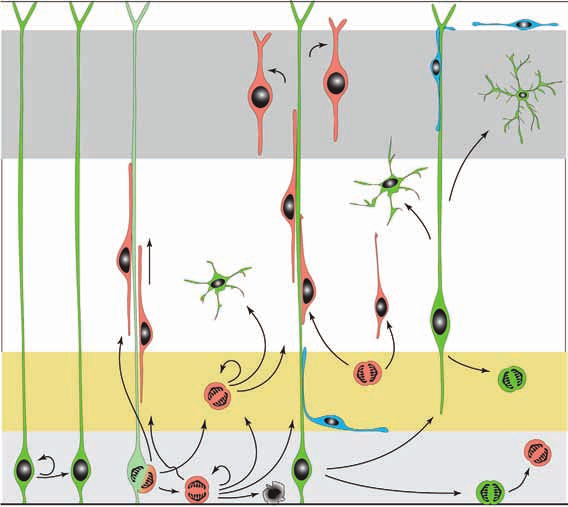
\includegraphics[width=0.8\textwidth]{rg_cells_division}\\
	\caption[A classical model of radial glial cells division processes \cite{Rakic2009}]{Illustration of a classical model of radial glial cells complex nonlinear division processes and neuronal migration \cite{Rakic2009}. From left to right: \acsp{npc} (green) originally divide symmetrically; During differentiation, \acsp{npc} become \acsp{rgc}, which divide asymmetrically, generating neurons or neural progenitor cells (orange). Neural progenitor cells eventually divide symmetrically into neurons. The majority of neurons in humans is produced by neuronal progenitors. A part of the generated neurons migrate radially towards the cortical plate, by attaching on the \acsp{rgc} projections; Eventually, after brain maturation, most \acsp{rgc} in humans undergo apoptosis (i.e. cell death) or generate neurons-supporting cells, such as astrocytes.}
	\label{fig:rgc}
\end{figure}


\subsection{The adult human cerebrum anatomic and functional properties}
 Human cerebrum is the center of sensations and thinking. The following excerpt provides a summarized anatomic \cite{Bear2016chapter7app} and functional \cite{Ferng2022} perspective.  As aforementioned, cerebrum is entirely produced  from the telencephalon during fetal development, with the telencephalic vesicles ending up becoming the two hemispheres, that remain connected through what is known as the \textbf{Corpus callosum}.  The side view of each hemisphere is named \textbf{lateral}, and the view of the inner side is called \textbf{medial}. The human cerebrum outer covering surface is called \textbf{cerebral cortex}, the region on which the current study focuses. The human cerebrum appears distinctly different from other organisms, mainly due to the \textbf{sulci} (i.e. grooves) and \textbf{gyri} (i.e. bumps), with them being the result of the tremendous expansion of the cerebral cortex surface area during fetal development, folding and wrinkling in order to fit the skull. The precise pattern of gyri and sulci varies significantly across populations, rendering the brain surface unique per individual. Under a biopsy dissection or a \ac{mri} scan, the cerebrum appears to consist of two distinctly colored types of matter, implying changes in composition and consistency; the gray matter, at the outer part of the cerebrum, which  contains the cell bodies, dendrites and the axon terminals, where all synapses are, and the white matter, at the inner part, made up of myelinated (i.e. biologically insulated) axons, which connect different parts of gray matter to each other (\autoref{fig:cerebissection}). Protective layers on top of the gray matter, called \textbf{meninges}, ensure that the brain does not come in contact with the outer bone, with the one attached on and marking the outer borders of the gray matter named \textbf{pial surface}. In this study, the midthickness surface is examined, a term referring to the surface halfway between the pial and white matter surface. 

\begin{figure}[H]
	\centering
	\begin{subfigure}{0.475\linewidth}
		
		\centering
		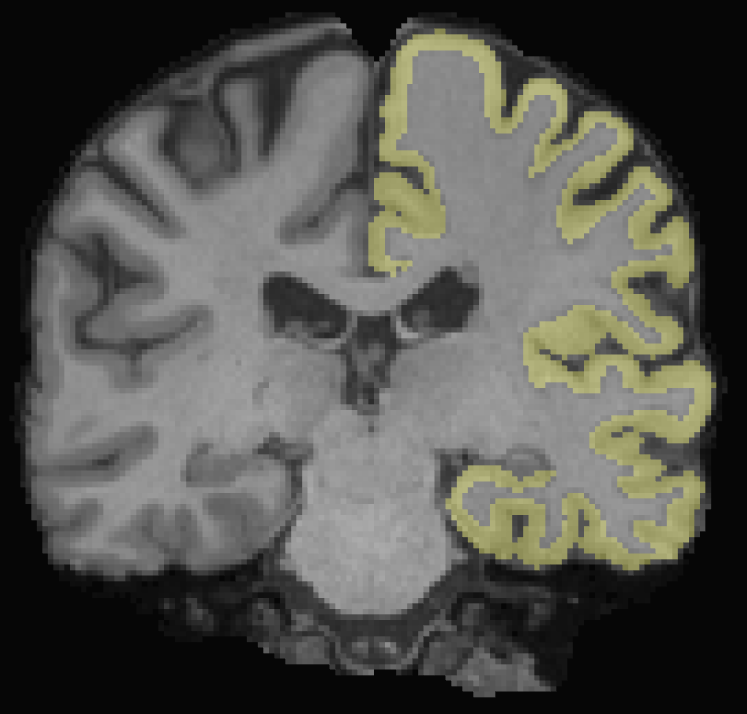
\includegraphics[width=0.475\linewidth]{coronal_section}
		\caption{Coronal section}
		\label{fig:coronal}
		
	\end{subfigure}
	\hfill
	\begin{subfigure}{0.475\linewidth}
		
		\centering
		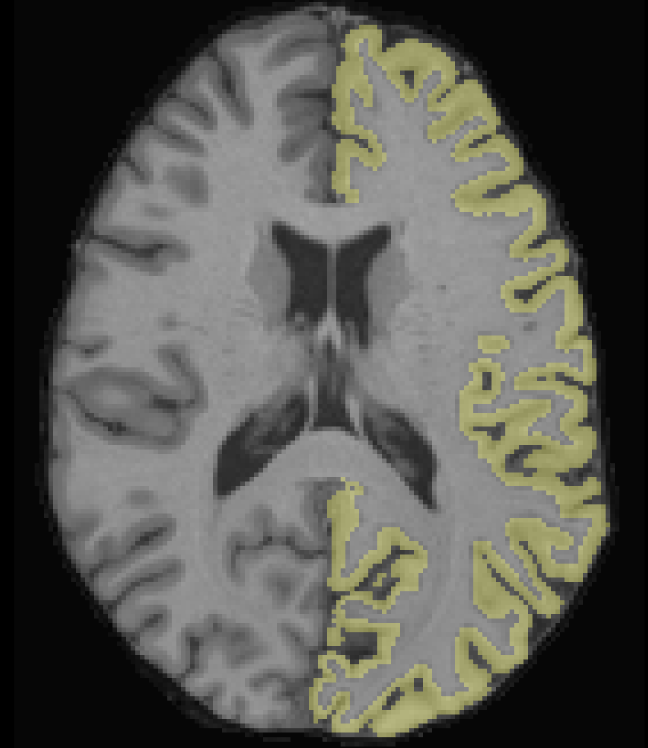
\includegraphics[width=0.475\linewidth]{axial_section}
		\caption{Axial section}
		\label{fig:axial}
	\end{subfigure}
	\vfill
	\begin{subfigure}{0.475\linewidth}
		
		\centering
		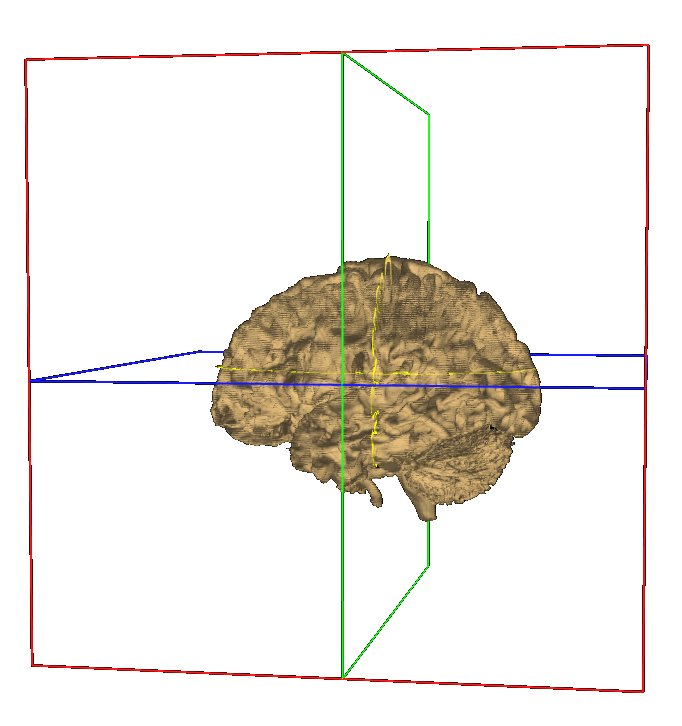
\includegraphics[width=0.475\linewidth]{3d_sections}
		\caption{\Ac{3d} sections map. Green rectangle corresponds to the coronal section plane (A) and
			blue rectangle to the axial section plane (B).}
	\end{subfigure}
	\caption[\Ac{mri} screening of gray and white matter]{Gray and white matter as seen from different sections, in an \ac{mri} screening, as retrieved from Freesurfer freeview routine. The gray matter is annotated with yellow color in the right hemisphere. Non brain regions have been removed.}
	\label{fig:cerebissection}
\end{figure}



\begin{figure}[H]
	\centering
	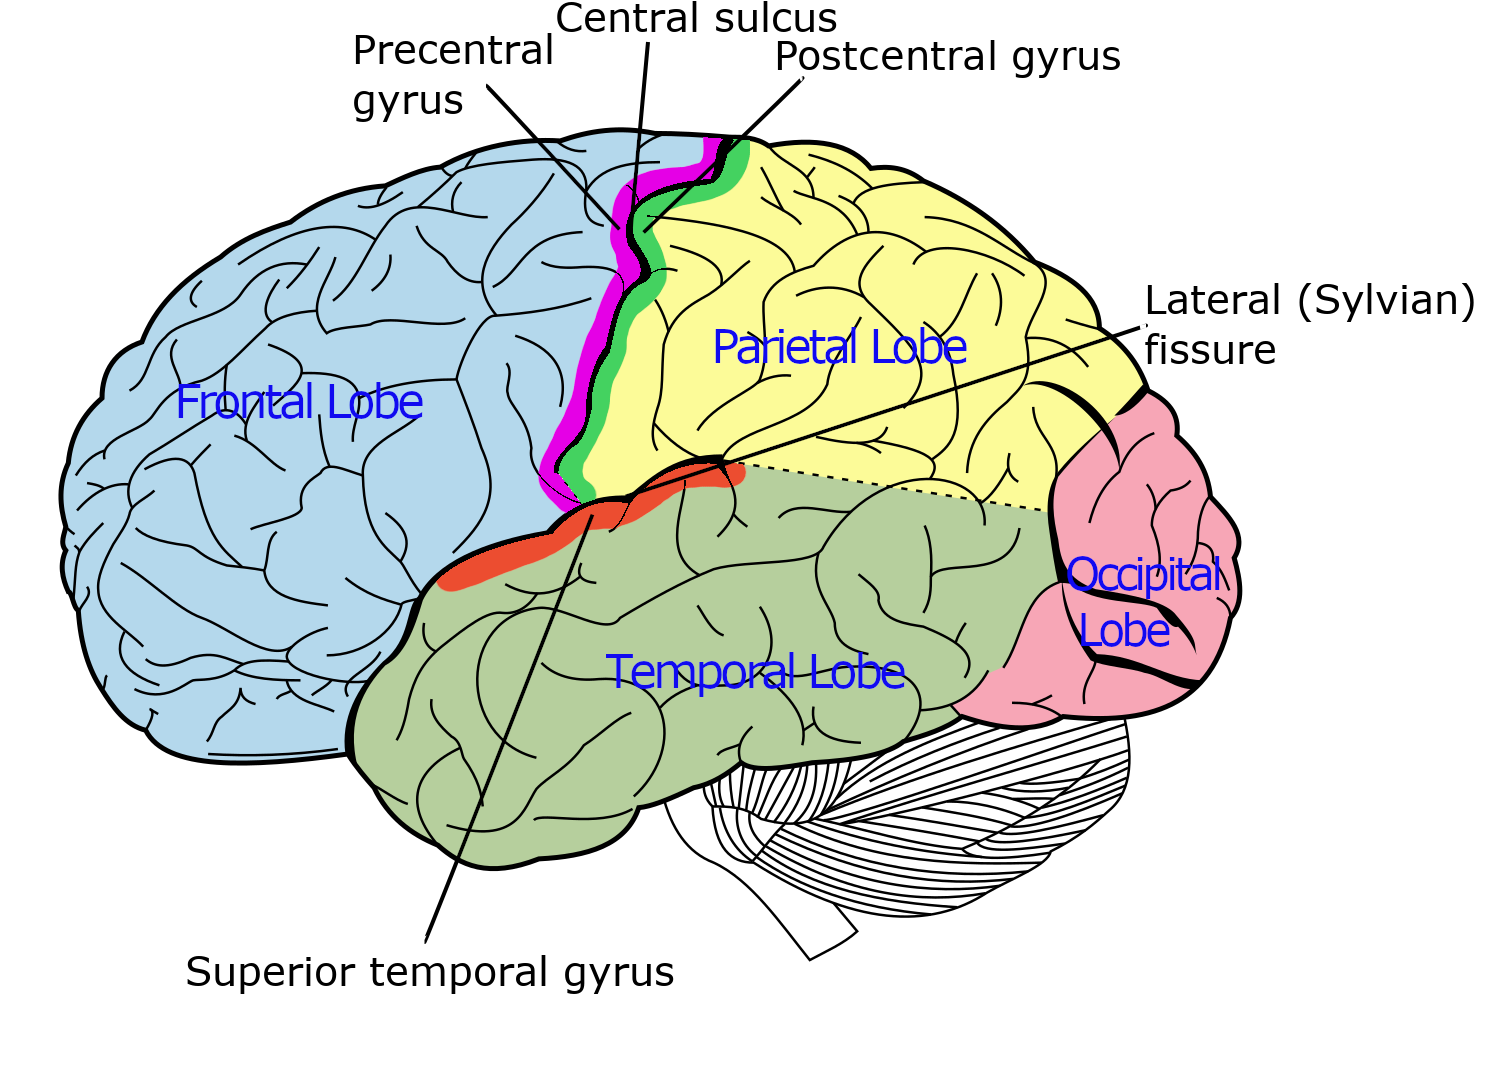
\includegraphics[width=0.8\textwidth]{1280px-Lobes_of_the_brain_NL.svg}
	\caption[A crude cerebrum partitioning]{Cerebrum lobes (blue font) and main gyri, sulci and fissures approximate positions (black font).}
	\label{fig:lobes}
\end{figure}

Efforts of partitioning the brain have been numerous throughout the years of medicine, with diverse resolution and purpose. Crudely, the cerebrum hemisphere is divided into lobes, that are named, by convention, after the bones of the skull that lie over them (\autoref{fig:lobes}).  A more detailed approach is based on the identification of the functional processes that take place in each part of the cortex, with Korbinian Brodmann being the first person constructing a 52-partitions experimentally based approximation of the hemisphere \cite{Brodmann1909} (\autoref{fig:corticalfunctions}). The main regions identified are:

\begin{figure}[H]
	\centering
	\begin{subfigure}{0.45\textwidth}
		\centering
		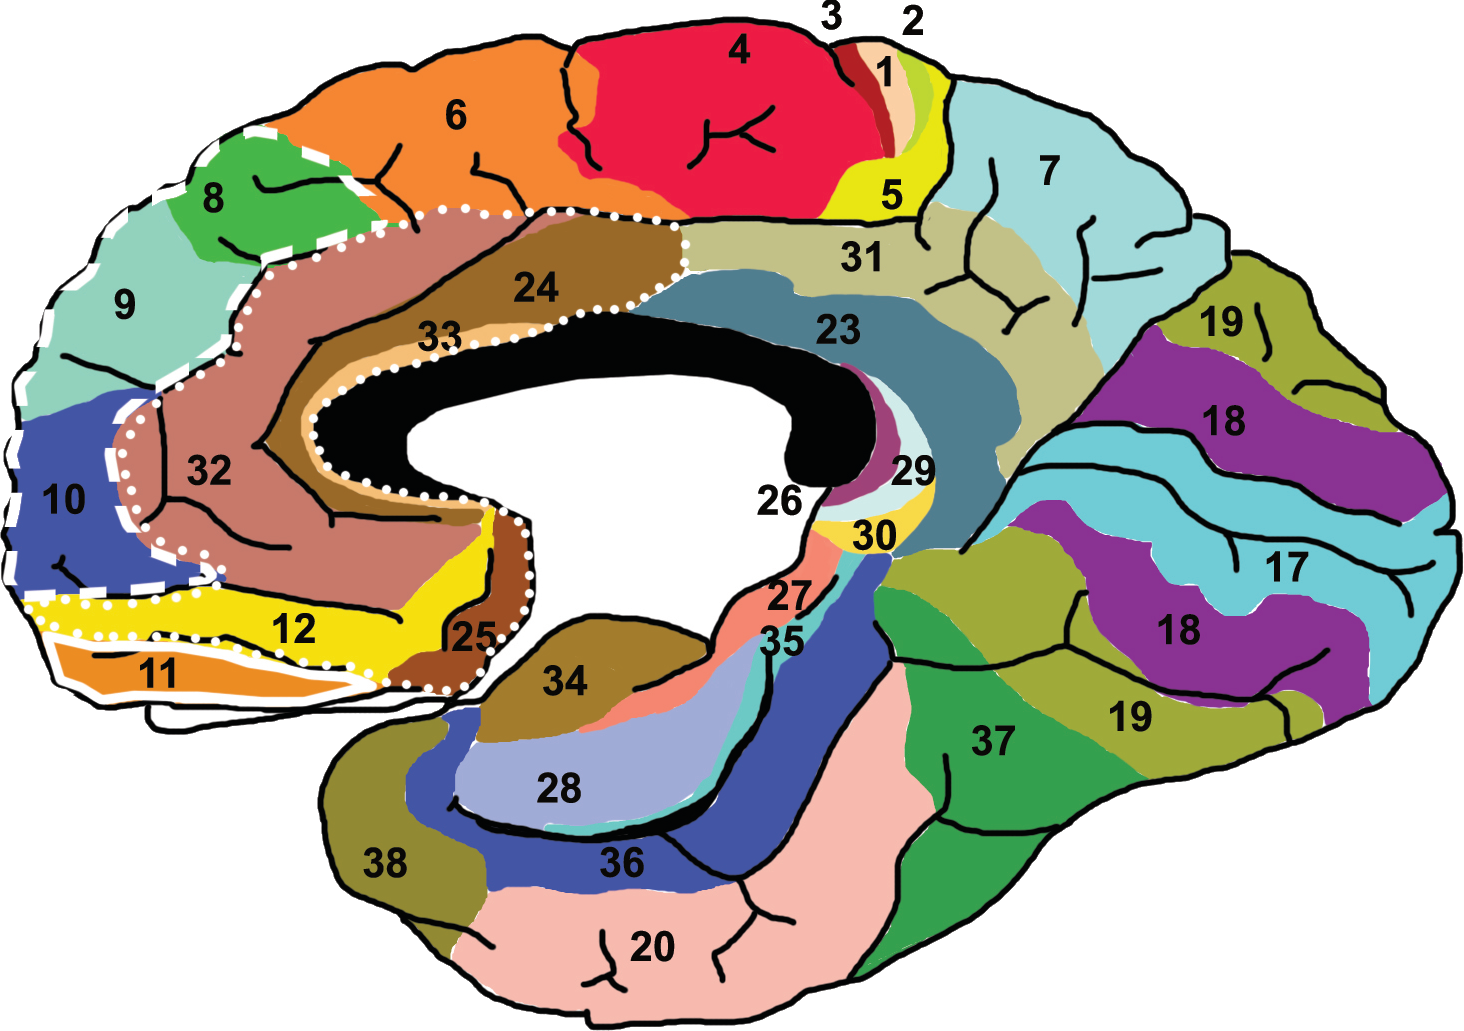
\includegraphics[width=\textwidth]{brodmann_medial}
		\caption{Medial surface}
		\label{fig:brodmann_medial}
	\end{subfigure}
	\hfill
	\begin{subfigure}{0.45\textwidth}
	\centering
	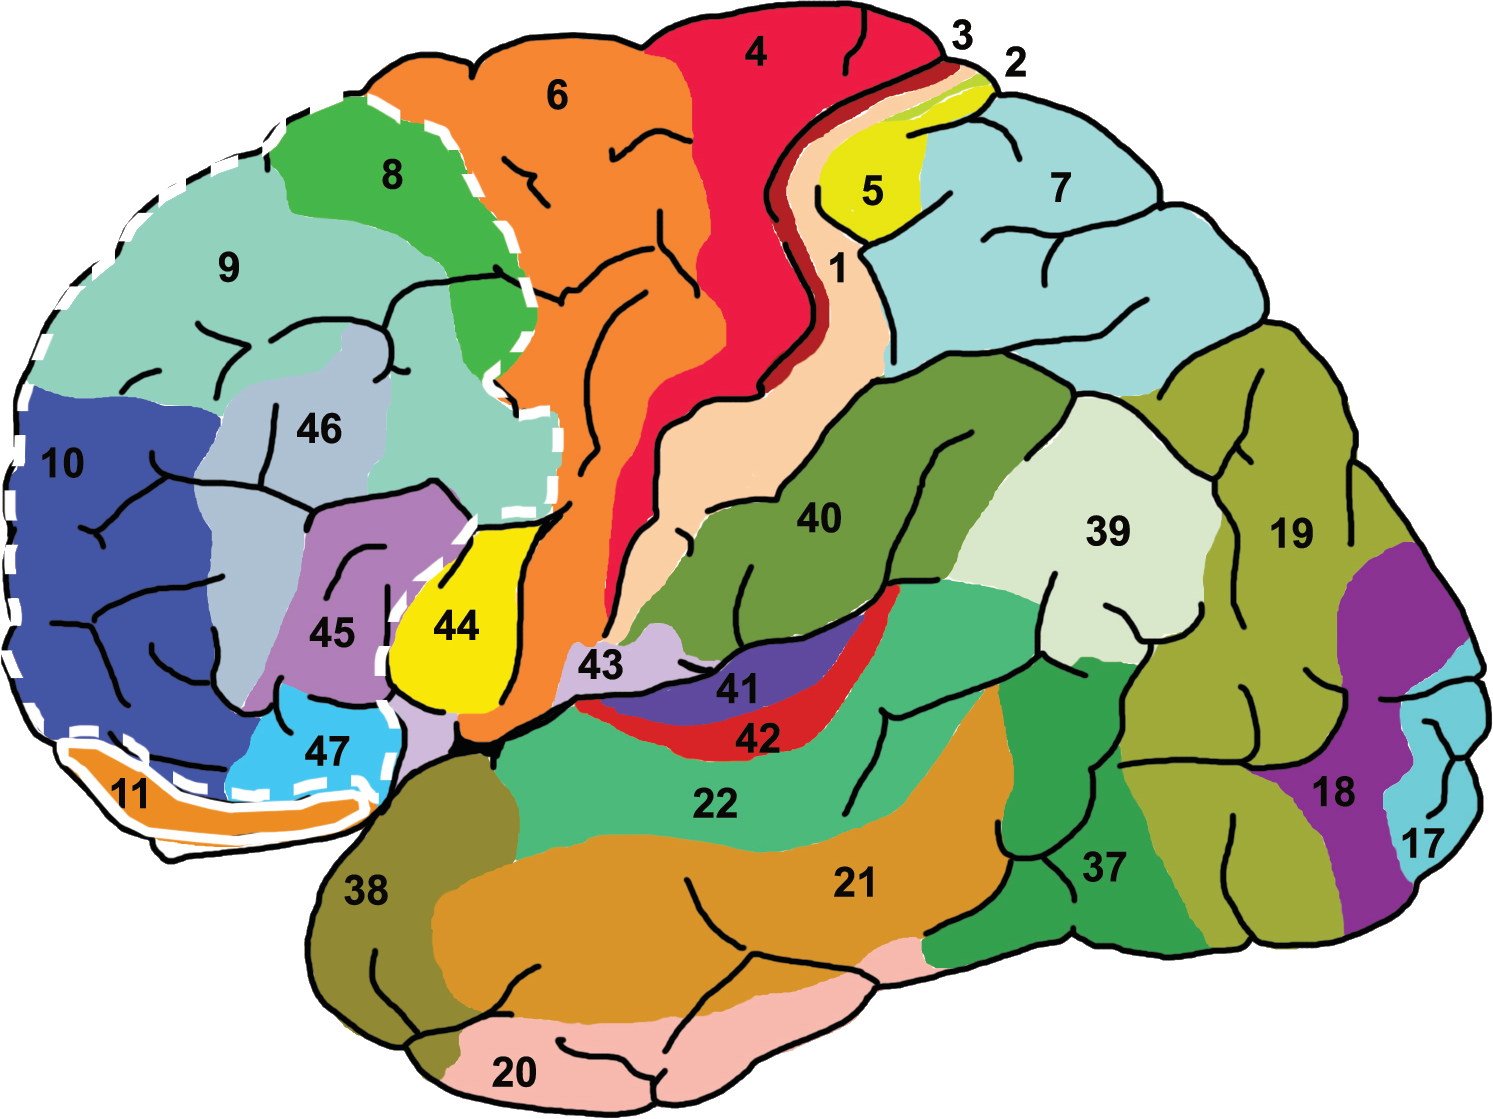
\includegraphics[width=\textwidth]{brodmann_lateral}
	\caption{Lateral surface}
	\label{fig:brodmann_lateral}
	
	\end{subfigure}
	\caption{Brodmann map of functional partitions.}
	\label{fig:corticalfunctions}
\end{figure}


\begin{itemize}

	\item{Sensory areas:
	\begin{itemize}
		\item {Somatosensory cortex (areas 1-3): the post-central gyrus (\autoref{fig:lobes}). It is responsible for the body-wide sensory information processing, such as touch, temperature and pain.}
		\item {Visual cortex (areas 17-19): occipital lobe surface. It constitutes the center of processing of visual information, as received from the optic nerve.}
		\item {Auditory cortex (areas 41,42): rostral posterior part of the temporal lobe. It processes auditory information, identifying fundamental sound characteristics, such as frequency and loudness.}
		\item {Gustatory cortex (area 43): An area behind the temporal lobe, responsible for taste signals processing.}
	\end{itemize}}

	\item{Motor areas, that are related to movement planning and manifestation:
	\begin{itemize}
		\item {Primary motor cortex (area 4): The precentral gyrus (\autoref{fig:lobes}). It is the center of voluntary movements execution, generating the electrical signals required for the neural impulses to be transmitted to the body muscles. }
		\item {Premotor cortex and supplementary motor area cortex (area 6): rostral part of the frontal lobe, anterior to the primary motor cortex. They are the center of motion planning and control, determining the sequence of movements required for a simple task to be performed.}
	\end{itemize}}
	\item{Association areas, which are related to perception, memory and thought processes:
	\begin{itemize}
		\item{Prefrontal cortex (areas 8-14,24,25,32,44-47): anterior part of the surface of the frontal lobe. It is centrally involved in cognitive control functions, spanning attention, salience detection, inhibitory control, working memory (i.e. short-term temporarily stored memory, related to a certain task), cognitive flexibility, empathy and pain processing \cite{Ong2019}. Areas 44 and 45, referred to as \textbf{Broca's region}, are responsible for speech production. Human prefrontal cortex remains one of the least functionally demystified parts of the cortex , presenting difficulties in every level of study, as it exhibits a higher relative size, higher cellular type variety, more complicated neuronal migration and denser connectivity patterns than other animals.\cite{Chini2021}}
		\item {Inferior temporal cortex (areas 20,21): caudal part of the temporal lobe cortex. It is responsible for the aggregation of the processed visual information towards a meaningful interpretation, supporting object recognition.}
		\item {Posterior parietal cortex (areas 5,7): posterior part of the parietal lobe surface. It processes sensory information produced from  all six senses to construct a semantic representation of the person's surroundings, leading to motion planning and spatial reasoning.}
		\item{Cingulate gyrus (areas 23-24,28,33): an arch-like fold rostrally to corpus callosum. It is the conscious part of the \textbf{limbic system}, which is the center of emotions, instinct and reflex responses.}
	\end{itemize}
}	
\end{itemize}

 Recently, with the advance of imaging methods, maps have been manufactured, to automatically partition the \ac{mri} extracted \ac{3d} cortical surface, based on morphological characteristics. One such gyral-based atlas, \ac{dk}, is derived from the changes in curvature under an expert-driven model of gyri locations \cite{Desikan2006} and provides automatic \textbf{cortical parcellation}, aligned to the Brodmann functional partitioning (\autoref{fig:dk}). This atlas is going to be used throughout the proceeding analysis for the quality control of applied segmentation techniques.
 
 \begin{figure}[H]
 	\centering
 	\includesvg[width=0.8\textwidth]{dk_left}\\
 	\caption[Desikan-Killiany atlas on midthickness surface]{\Acl{dk} atlas, mapped on the midthickness surface of the left hemisphere, with the medial (left) and the lateral (right) views displayed.\cite{Dickie2019} Different colors represent different partitions. The black region has not been mapped.}
 	\label{fig:dk}
 \end{figure}
 
 
 
\subsection{Reported general human cortex symmetry traits}
Although human cortex exhibits roughly symmetric structure, the symmetry is systematically suppressed, not only due to the environment, with plasticity playing central role, but also because of genetic factors, as explained in the previous sections. An asymmetric pattern is manifested across adult individuals, irrelevantly of their upbringing, comprising, therefore, a characteristic of the human species, while general abnormalities in this pattern are related to the occurrence of mental disorders, such as autism or developmental language disorder \cite{Herbert2005}\cite{Kong2022}. Some of the most prominent asymmetric traits across healthy individuals are the following:
\begin{itemize}
	\item{Yakovlevian torque (\autoref{fig:yaktorque}): the right hemisphere prefrontal lobe and the left hemisphere occipital lobe tend to cross the midsagittal plane, extending towards the other hemisphere \cite{Kuo2022}. This creates a phenomenon of counter-clockwise warping, making the whole brain appear slightly leftwards rotated, while also making an impression on the inner part of the skull, called \textbf{petalia}. Increased left hemisphere occipital lobe extension, possibly caused by enlarged left lateral ventricle, is correlated with bipolar disorder\cite{Maller2015}. Rising absence of the torque during aging is connected to schizophrenia  and other mental disorders \cite{Ribolsi2014}.}
	\item{Peri-Sylvian asymmetry: the left Sylvian (lateral) fissure is longer and sharper than the right one, while the right Sylvian fissure exhibits a more visible leftward curve, in the part where temporal lobe meets the parietal lobe, that is the auditory cortex, also called \textbf{planum temporale} \cite{Kuo2022}. The increased thickness of the right superior temporal lobe, that reduces the lateral fissure steepness, is attributed to increased white matter volume. Such trait has been reported to be gender-related, with males exhibiting greater asymmetry than females, as noted in previous studies, with steroid hormone receptor activity and steroid metabolic process related genes \cite{Guadalupe2015}.}
	\item{Central sulcus asymmetry: the right hemisphere central sulcus is deeper and larger \cite{Kuo2022}. Larger asymmetry appears to be correlated with \ac{adhd} \cite{Li2015}.}
	\item{Motor areas asymmetry: the motor areas are generally larger on the left hemisphere.}
\end{itemize}

Statistical modeling of the observed symmetry pattern can provide a hint on the significance  of genetic and environmental factors contribution\cite{Klingenberg2020}. The current study focuses on the genetic component, which has been diversely investigated across literature.


\begin{figure}
	\centering
%	\begin{subfigure}[t]{0.45\textwidth}
%		\centering
%		\includesvg[width=0.9\textwidth]{demoTorqueBrainAsymmetry/STAGE00DATA/averaged_torque_0_468}
%		\caption{Computed approximation of the Yakovlevian torque from working dataset, showing succinct clockwise rotation of 0.47 degrees (red line) versus the vertical black line.}
%		\label{fig:yakovlevian_computed}	
%	\end{subfigure}
%	\hfill
%	\begin{subfigure}[t]{0.45\textwidth}
\centering
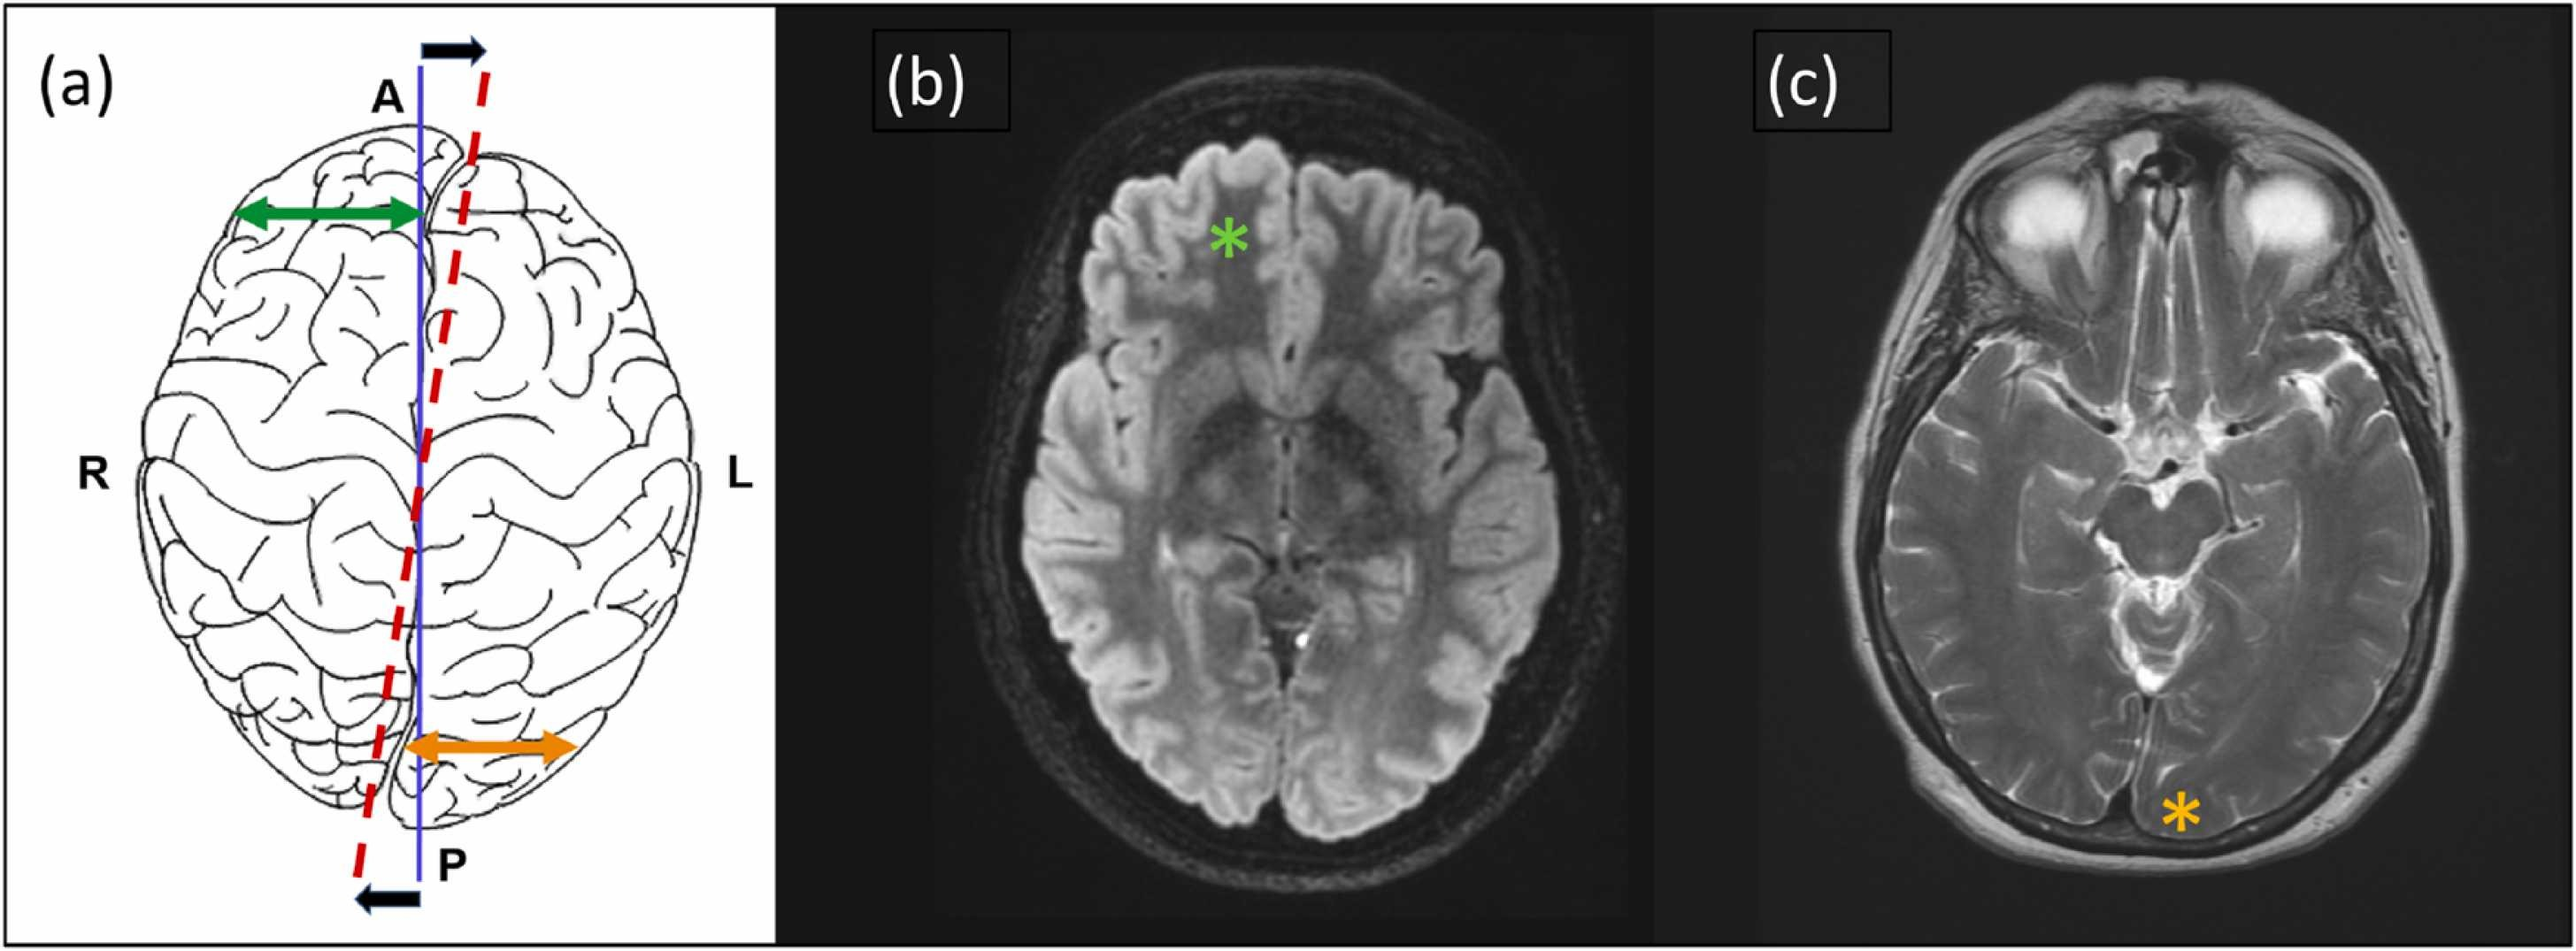
\includegraphics[width=\textwidth]{yakovlevian_external}
\caption[Yakovlevian Torque \cite{Kuo2022}]{Yakovlevian torque schematically illustrated (a), along with its manifestation in different axial sections for a single individual (b,c) \cite{Kuo2022}.}
%		\label{fig:yakovlevian_external}
%	\end{subfigure}
%\caption[Yakovlevian Torque \cite{Kuo2022}]{Illustration of the Yakovlevian torque. The angle of rotation in (A) was calculated by using the average angle of the longest edges, close to the midsagittal plane, of the convex hulls of the horizontal plane projection of each hemisphere midthickness surface, after shape normalization (see \autoref{subsec:shape_normalization}), per individual, across the studied population.}
\label{fig:yaktorque}
\end{figure}



\section{Genetics of multivariate quantitative traits}

\subsection{\Acf{mvgwas}}
\Ac{gwas} aim to relate genetic information, usually extracted from \acfp{snp} markers arrays, with a phenotypic trait. When the trait is dichotomous, measured as presence or absence of a certain quality, then \ac{gwas} are applied on a case-control fashion, where two cohorts, one exhibiting (case) the trait and another not (control), are compared. \cite{Uffelmann2021} In the present work, the focus is directed to quantitative traits, whose measurement takes continuous values.

\Acfp{snp} are characterized by single nucleotide base-pairs positions where two or more different alleles (i.e. variants of nucleotide bases) are observed, with the second most frequent allele appearing with a frequency, called \ac{maf}, higher than 1\%, a property that sets this term apart from the more general notion of a single-nucleotide variant. Being the most common type of polymorphism in the human genome, \acp{snp} were popularized on account of their considerable effect on influencing transcription. Apart from the direct case, where a \ac{snp} belongs to an exon and the alternate allele corresponds to a non-synonymous (the translated amino-acid differs) or a nonsense (the codon stops translation) mutation \cite{Ramensky2002}, the majority of registered \acp{snp} (88\%) reside in non-coding regions. They can have an impact on the physio-chemical properties and conformation of docking positions for \ac{dna}-binding enzymes, such as \acp{tf}, causing binding affinity changes, influencing transcription regulation and, ultimately, altering biological pathways relevant to dependent phenotypic traits \cite{Nishizaki2020}. As a matter of fact, 31\% of the known \ac{dna} elements, as reported by the ENCODE project, the human genome encyclopedia, appear to be part of \acp{tf} binding domains \cite{Dunham2012}.

Phenotypic differences among individuals, described by the trait variance $V_p$,  are the result of genetic variation $V_g$, known as \textbf{heritability}, environmentally induced variation $V_e$ and developmental noise $V_d$ (the deviations observed when environment and genetics are controlled), formally denoted as $V_p=V_g+V_e+V_d$ \cite{Vogt2020}. The genetic information content $V_g$ is \textit{approximated} by the amount of variation the alleles occurrence of a certain subset of \acp{snp} translated to variation in the studied trait properties.  The presence of a minor allele signifies divergence from the general population characteristics, and hence implies that information is contained in that \ac{snp}.  The relationship of each \ac{snp} with the phenotypic trait is statistically represented by a certain genetic model. Under the assumption of an \textbf{additive model}, if a certain minor allele occurs in both \ac{dna} strands, i.e the allele is homozygous at that locus, then its effect is double compared to the heterozygous case, independently of which strand is carrying it. This hypothesis requires no prior knowledge and makes no further assumptions regarding the alleles dynamics, that is the degree of dominance of each allelic variant. The described model, for a single quantitative trait (dependent variable) and a \ac{snp} with a single minor allele (assumed independent variable) can be formulated using a univariate linear regression $y = \beta x$, with $y$, ranging from 0 to 2, being the number of the allelic occurrences, $x$ being the phenotypic trait and $\beta$ the \ac{snp} effect. A \ac{snp} is then considered to have significant effect on the trait, if its calculated effect and the effective population size contradicts the null hypothesis $H_0$ of no association given an arbitrary probability cutoff \cite{AlejandroGonzalez-Chica2015}. Low sample size affects the type I error of the detection, namely the presence of false negatives that confirm the alternate hypothesis. $H_0$ is represented by a $\chi^2$ distribution with 1 \ac{dof}. The probability threshold is derived based on an empirical value, fixed to 0.05, corrected using the Bonferroni correction for multiple independent tests, hence $\frac{0.05}{N_t}$ with $N_t$ the number of \acp{snp}. The method is rather conservative, therefore usually cutoffs are computed by replacing the number of tests with the amount of independent common \acp{snp} for a given population. Based on the findings of the International Hapmap Project, this amounts approximately between 200,000 to 1 million \textbf{tag} \acp{snp}, i.e. \acp{snp} that are representative in high \ac{ld} regions, where non-random association of genetic loci is prevalent \cite{Belmont2003}. Therefore, the cutoff threshold $5\times 10 ^ {-8}$ is used. The p-values are most commonly converted to values proportional to significance, by applying the $-\log_{10}{p}$ transformation.   The \ac{ld} phenomenon, often locally observable, causes seemingly continuous p-value spikes to appear when plotting the data points, with the lead, or functional, \ac{snp}, the one with the greatest local significance (i.e. the lowest locally recorded p-value), being `supported` by lesser significant \ac{snp} in its surroundings, producing as a result a scatter plot that resembles the Manhattan city landscape (\autoref{fig:gwas_example}).

 \begin{figure}[H]
 	\begin{subfigure}[t]{0.45\textwidth}
	\centering
	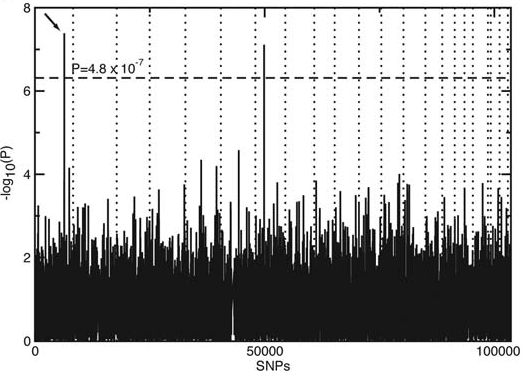
\includegraphics[width=0.9\textwidth]{gwas_2005}
	\caption{}
	\label{fig:gwas_2005}
	\end{subfigure}
	\hfill
	\begin{subfigure}[t]{0.6\textwidth}
		\centering
		\includesvg[width=0.9\textwidth]{asymmetry/genomeDemo/STAGE00DATA/not_imputed/not_subsampled/gwas.svg}
		\caption{}
		\label{fig:gwas_example}
	\end{subfigure}
	\caption[Examples of GWAS Manhattan plots \cite{Klein2005}]{Examples of \ac{gwas}. In (A), the first recorded \ac{gwas} Manhattan plot \cite{Klein2005} is displayed, where a single \ac{snp}, related to Complement H Factor Polymorphism, was identified to affect age-related macular degeneration disease propensity, one of the major causes of blindness among elderly. In (B), a \ac{gwas} scatter plot from the present work is shown, where the \acp{snp} spikes signal is evident, attributed to \ac{ld}.}
	
\end{figure}



There are several design benefits and limitations of such a process. \ac{gwas} have been successful in revealing novel relationships between genes with known properties and a variety of observed phenotypic traits and clinical applications, presenting evidence of possible biological mechanisms related to genes with unknown function \cite{Tam2019}. They also empower population-specific comparative studies, at the level of how ethnicity or other kinds of population stratification affect a certain trait, while accommodating the possibility to investigate the effect of an allele no matter how frequently it might appear in the studied sample \cite{Tam2019}. On the other hand, it has been generally observed  that each \ac{snp} can only explain a small part of the heritability of a certain trait, with a large amount of the signal hidden in gene-to-gene interactions, that are not captured in this method, and possibly in \acp{snp} whose contribution has not been considered significant enough. To remedy the latter issue, larger sample size is ideally required. TO BE CONTINUED/FIXED



However, the analyzed phenotype is described by more than one properties, that are related to the different landmarks composing the cortex of each individual. Also, a single \ac{snp} may exhibit more than one minor allele. The goal in this study, consequently, is to incorporate multi-allelic \acsp{snp} and, more importantly, multivariate phenotype, in a single hypothesis test per \ac{snp}, leading to what is called \ac{mvgwas}. In general, there is an abundance of strategies on how to perform \ac{mvgwas}, ranging from direct methods, that approximate the inputs relation either in an unbiased manner or making certain educated guesses, to more complex techniques, that increase statistical power by transforming the inputs, at the expense of explanatory ability \cite{Galesloot2014}. There are also methods that are based on the meta-analysis of outcomes from univariate studies, commonly used to juxtapose experiments from separate sources, for which the original data is missing, the experimental setup across studies is significantly different or a single study is computationally intractable \cite{Uffelmann2021,Cichonska2016}. Which approach performs best mainly lies on the dataset properties and the nature of the scientific question. Factors such as low sample size \cite{Sheng2021}, genes pleiotropic effects \cite{Fernandes2021} (i.e genes interacting through seemingly independent biological pathways) or within-study variability \cite{Usui2021,Jackson2011} tend to handicap the statistical modeling and increase the type I and II errors of the corresponding hypothesis tests. 





In this study, \ac{cca} was primarily chosen due to the high capacity in efficiently reducing the inputs dimensionality while preserving most information regarding their correlation. Diverse experiments, analyzed in \autoref{chap:gwas}, have been applied to identify the method that gives high fidelity results, consistent with relevant literature. The analysis outcome requires further processing, as explained in \autoref{sec:postprocessing}, to account for the main weakness of this method, that it does not consider the \ac{snp}-to-\ac{snp} effect, tackled using as proxy the notion of \ac{ld}, and subsequently to topologically and functionally enhance the filtered findings. Once this additional step has been performed, a cross-traits analysis is applied, described in \autoref{sec:metaanalysis}, where the \ac{da} genetic signature is compared with the signatures of phenotypic traits, analyzed in a similar study \cite{Naqvi2021}, the cerebral and facial shapes.





\section{Phenotypic trait analysis}\label{sec:phenotype_intro}
\subsection{Summary on cortex anatomy}
 
\subsection{Dataset Description}
 

The current study focuses on identifying the genetic landscape that composes the observed symmetry pattern, hence, subsequently, a brief introduction into how the genetic variations are being statistically modeled is provided.




\citet{Sha2021}


\subsection{Phenotypic partitioning}\label{sec:hsc}
\Acf{hsc} is an unsupervised method of iterative partitioning, that makes use of the distance matrix eigenvectors \cite{Ng2002}. It results into a binary tree structure (i.e. each parent shape is partitioned into two children). In the current study, a level-4 partitioning is performed, resulting into 31 partitions. Subsequently, they are transformed to the corresponding principal components that explain 80\% of the variance, for reasons of further dimensionality reduction. TO BE CONTINUED




\section{Breaking the complexity into parts}
TO BE EXPANDED

The present work evaluates the brain asymmetry genetic landscape in a coarse-to-fine segmentation, through the application of \ac{hsc}\cite{Ng2002}, discussed in \autoref{sec:hsc}. The technique has been used in a number of different related studies \cite{Claes2018}\cite{Naqvi2021}, yielding results that are in accordance with the underlying anatomic features. The main reason behind this partitioning is the intrinsic complexity of the studied phenotype, eliciting expected differences in the genomic profiles of each cerebral cortex region. The basic assumption made is that topologically close landmarks share similar genetic background. In general though, this type of distance-based clustering is governed by the least quantity of assumptions, regarding the shape or form of the cluster \cite{VonLuxburg2007}. The partitions' genetic juxtaposition is valuable for identifying which regions share similar significant genetic loci, highlighting the corresponding genes contribution, or showcasing the specialization of certain regions that share little to no similarities with their neighbors. Identifying the latter provides a way of mapping the developmental activation of each locus, bringing forth the opportunity to augment the results of related developmental studies \cite{Vijayakumar2016}.

\section{Searching for the origin}
TO BE EXPANDED

The genomic studies are performed under the framework of \ac{snp}-by-\ac{snp} \ac{cca}. 


\section{Data description}
In this study, targeted on humans, a cross section between the dependent cerebral asymmetry and the independent genetic factors is performed, in an effort to discover affiliated genetic regions and provide a novel understanding of the related genes cooperation. With the advent of technology capable to collect and process genomes from different individuals in relatively high speed, vast databases have been constructed. One of the main players in the data collection has been UK Biobank; a large-scale database from a randomized consortium of 500,000 individuals, whose genome has been collected, from whom  48,000 subjects had also participated in brain \ac{mri} collection process, as of December 2020 \cite{Littlejohns2020}. In this thesis, we exploit this newly acquired dataset to identify the key loci that are related to the human brain surface symmetry. Only healthy self-proclaimed white European individuals were considered. 

\section{Novelties based on related literature} 
 Due to the biological importance of cerebral bilateral asymmetry, it is a subject that has been rigorously studied from multiple viewpoints.
 \subsection{Evolution}
 From an evolutionary stand, it is extremely rare for the right conditions to occur, in order for any soft tissue specimen to be preserved, across a considerable amount of time. The only known way is through mineralization \cite{Purnell2018}. This fact renders a mammal's ancestor brain almost impossible to retrieve. Nevertheless, endocranial imprints have been used as a proxy to describe the relationships between hominids and their ancestors \cite{Balzeau2012}\cite{Neubauer2020}. The reason behind this phenotypic delegation is purely practical. The brain size and shape follow the container volume restrictions. Although such studies support the theory of propagating asymmetry among studied individuals, with the most evident signs of \ac{da} in human skulls, little information about the surface shape can be retrieved, as only the convex hull shape of the brain can be delineated from such process. Through the association of brain asymmetry with \acs{dna}, a universal code among organisms, it becomes possible to deploy tools used by evolutionary geneticists, to identify the phylogenetic tree of this complex trait, locating conserved regions among organisms and their predicted divergence in time, under a pleiotropic model \cite{Koch2021}.
 \subsection{Clinical studies}
 
\chapter{Materials and Methods}\label{chap:mat_and_methods}
In figure \ref{} a brief overview of the processes applied in this work is displayed. In the coming sections, each compartment will be separately analyzed.

\begin{figure}
	content...
\end{figure}


\section{Data description}
\subsection{Primary Data Source}
With the advent of technology capable to collect and process genomes from different individuals in relatively high speed, vast databases targeting human physiology have been constructed. One of the main players in the data collection has been UK Biobank; a large-scale database from a randomized consortium of 500,000 individuals, whose genome has been collected, from whom  48,000 subjects had also participated in brain \ac{mri} collection process, as of December 2020 \cite{Littlejohns2020}. Participants were male and female, with the age range spanning 40 to 69. The study focuses on healthy self-reported white individuals of European ancestry, filtering and preprocessing them based on the work of \citet{Naqvi2021}. Specifically, the discovery dataset, amounting to 19,644 individuals, of the present work was identical to the one used in their study. In addition to that data, a smaller one, coming from a different, collected at a later time, batch, of 16,342 individuals was used as a replication dataset during \ac{gwas}, reapplying with the same filtering and preprocessing steps. More information about the signal-specific preprocessing is provided in the next sections.


\section{Methods applied on Phenotype}
\subsection{Initial filtering and preprocessing}
\label{subsec:pheno_preproc}
T1-weighted MRI scans are analyzed. The analysis is performed by initially converting the raw DCIM MRI volumetric images to well-defined 3D surface triangular meshes through the pipeline applied by FreeSurfer `recon-all` \cite{Reuter2012} and ciftify `ciftify-recon-all` commands \cite{Dickie2019}, on a space of 32 thousand vertices, with the average edge length being 2mm. Subsequently, the mid-cortical surface is arbitrarily selected, purportedly because of its plausible smoothness, allowing the distinction of sulci and gyri without over-representing their geometry \cite{Naqvi2021}. After quality control,  the vertices from the sub-cortical part of the surface, referring to corpus callosum connection points, were removed based on a mask derived from the Conte69 atlas \cite{Glasser2011}, getting reduced to 29,759.

\subsection{\Ac{mri} Shapes Normalization}\label{subsec:shape_normalization}
The current work applies principles from general symmetry studies to model cortical asymmetry. For any of these analyses to occur, the abberations of \ac{3d} shapes produced from \ac{mri} scans need to be considered. \Ac{mri} output is affected by the subject positioning and technical error \cite{Wittens2021}.  Volumetric differences also increase the level of discrepancies among \ac{mri} samples.  To prevent positioning and volume deviations from gravely affecting shape comparisons, a normalization is required\cite{Klingenberg2020}. The samples of the derived 3D triangular mesh are represented as a set of vertices $\mathcal{V_S}$ of predefined dimensionality P, with a single landmark coded in the format of (x,y,z) coordinates. Those are joined together with a predefined faces matrix $\mathcal{E_S}$, with each of its elements containing three indices referring to $\mathcal{V_S}$, with the additional constraint that $S$ is a multiple-connected structure, namely a graph in which there is at least one path joining any two vertices. Shapes normalization is performed through the application of \ac{gpa}. \Ac{gpa} is an algorithm that iteratively performs translation, scaling and rotation on a given set of structures $S$, given initially a reference $S_0$, aiming to minimize the euclidean distance of corresponding points and the average shape. The translation is performed in such a way that the centroid C, defined by $\frac{\sum_{\forall i}{\mathcal{G_S}}_i}{P}$, becomes the system origin. The scaling is such that the centroid size of the normalized $S$ structure, defined by $\sqrt{\sum_{\forall i}{\left|\left|{\mathcal{G_S}}_i-C\right|\right|_2}}$ becomes equal to 1. The transformed samples then belong to what it has been coined as Kendall Space \cite{Klingenberg2020}.  Under the framework of cortical surface analysis, a single hemisphere is considered to be one of the $S$ structures. To apply any symmetry analysis, therefore, one of the individual hemispheres needs to be mirrored on the other side of the midsagittal plane, and then \ac{gpa} is applied to align all hemispheres at once. The mirroring is performed by normalization of right and left hemispheres sets separately, and, then, x coordinate sign inversion of the right hemisphere landmarks. Aligning, finally, the entire dataset marks the end of the shapes normalization for the two tasks, statistical asymmetry analysis and \ac{gwas}.

\subsection{Shape downsampling}
\label{subsec:downsampling}
An intermediate step is followed when performing corticla symmetry statistical analysis, in order to reduce the computational burden of the process. A rather simple algorithm, in MATLAB context, has been derived, that computes the subset of indices of a given shape S, \textit{approximately} with a given factor, that best describe the downsampled shape $M$ provided from the  proprietary function `reducepatch` output \cite{Lopez2014}. From this method, the analyzed shapes were downsampled by a factor of 10, with the average shape retaining most morphological characteristics. The key idea is to find the one-to-many correspondence between faces from the two meshes. Let $\mathbf{{Cn}_T}$ be the centroids of each face of a shape T. The faces correspondence is found by identifying for each face $x\in G_M$ with index $i_x$ a part $S_x$ of S with $\mathcal{G_{S_x}}\subset G_S$ joined through a path length of 10, given the desired reduction rate to the closest face $y_{min}(x)=argmin_{\mathbf{{Cn}_Y}}\left|\left|\mathbf{{Cn}_Y}-\mathbf{{Cn}_M}\right|\right|$. Those elements are having non-zero entries in the 10th power of the S's adjacency matrix, at the $y_min$-th row. Then, the optimal vertex correspondence is found by taking all the vertices corresponding to the faces subset $\mathbf{V_{S_x}}$ and identifying which of them is the closest to each of the vertices of x. The resulting downsampled shape R then has the faces of M, but projected on the vertices of S. This mapping allows for instant, although naive and of reduced quality, downsampling of 29,759 to 3,098 landmarks (\autoref{fig:downsampling}).
\begin{figure}[H]
	\centering
	\includesvg[width=\linewidth]{downsampling/reduction}
	\caption{Downsampling indices of original average template using the novel algorithm and specific reduction scales (1/r). As no inter-face edge connectivity criterion is being considered, artifacts occur in the approximated shape, in the form of scars.}
	\label{fig:downsampling}
\end{figure}

\subsection{Symmetry Statistical analysis}
Bilateral asymmetry is mainly described using three components in literature \cite{klingenberg2002}\cite{Vingerhoets2021}. \Acf{da}, the main focus of this study, corresponds to the hemispheric side effect, namely how the intrinsic (i.e. genetic) properties of the studied population are manifesting across individuals. Antisymmetry, which is related to the effect where sidedness is random in a population (i.e. left-right pattern is mirrored to a right-left pattern), is not observed in the human cerebral cortex, in contrast to other internal organs positions, or organisms \cite{Neubauer2020}. The third component, \acf{fa}, encompasses any random developmental and environmental effects, that cannot be explained with the existing knowledge. The observed deviations can be statistically linearly modeled as products of two effects, the hemisphere side studied and the individual specimen analyzed, as well as their interaction \cite{klingenberg2002}. Formally, based on \cite{VanDongen1999} assuming the presence of replications for each observation per individual, to account for technical error, a mixed linear model representing the aforementioned dependencies is defined as:
\begin{equation}
Y_{ijk} = \mu + \beta + I_i + S_{ij} + E_{ijk}
\end{equation}
where $Y_{ijk}$ is the phenotype of the i-th individual, from the j-th side, under the k-th replication, $\mu$ and $\beta$ are the fixed intercept and fixed side effect respectively, $I_i\sim\mathcal{N}(0,\sigma^2_{ind})$ is the random individual effect,  $S_{ij}\sim\mathcal{N}(0,\sigma^2_{FA})$ is the random side and individual specific effect, matched to \ac{fa}, and $E_{ijk}\sim\mathcal{N}(0,\sigma^2_{ME})$ is the measurement error. Given this definition, a way to measure the statistical significance is performed through an F-test applied on a 2-way nonparametric permutation-based \ac{anova}, to relate the \ac{rss} ratios of effects to observable error terms, and of fluctuating effect to the measurement error. 

While simple \ac{anova} bases the significance of the result on the assumption of normality, permutation-based \ac{anova} makes no assumptions on the underlying distribution \cite{Anderson2001}. Instead it bases significance of a F-score on the number of permutations which resulted in F-scores higher than the F-score measured in the simple \ac{anova} scenario on the original data, divided by the total number of permutations \cite{Klingenberg1998}. Let N be the number of individuals. A reshaping operation is performed, after which the set of size L landmarks becomes a set of size 3L coordinates per individual per side, in other words a \ac{3d} dataset. The permutations were generated considering each time the dimension being investigated, pursuing biologically feasible result when possible; for assessing the individual effect, the hemispheres were randomly shuffled across individuals; for the side effect test, landmarks of each individual were reassigned a random side; for the fluctuating effect, the whole dataset was randomly permuted. As it can be foreseen, a handicap of the latter permutation is that is being sampled from a possible set of $(6NL)!$ configurations, whereas the two former ones from $(3NL)!$ and $(6L)!$ configurations respectively. This renders the last test more sensitive to assign low p-values to each landmark, as the possible configuration that could possibly produce a better f-score is less likely to be selected. However, it is worth noting that in all tests the possible cases number is prohibitively large, and that analyses in Monte Carlo simulations suggest the size of 1000 replications as good enough \cite{Marozzi2004}. The consecutive analysis has also been demonstrated in the work of \citet{Vanbiervliet2022}. 1000 replications were, therefore, selected to test the significance of each asymmetry component, which means that the analysis was computationally intensive, but facilitated by the downsampling described in \autoref{subsec:downsampling}. Five random subsets of 50 samples were collected from the discovery dataset. The number of samples was chosen experimentally, as it was observed that the size of 1000 replications is actually not enough for larger datasets and the method was generally sensitive in assigning high significance (p-value<0.05) to each landmark, the larger the set size assessed. A number of different random subsets was selected, so that to reduce the effect of cherry-picking. The final counts were computed to be the average of the experimental iterations. Although the last step is not theoretically correct, as independent pools of combinations are assessed, it achieves a smoothing operation CITATION NEEDED.

Replications are necessary in such analysis, in order to distinguish the \ac{fa} effect from measurement error. To this end, an \ac{mri} test-retest subset of 20 individuals from HCP was retrieved \cite{VanEssen2013}, and the preprocessing mentioned in \autoref{subsec:pheno_preproc} was performed. For each landmark and coordinate, and for each hemisphere separately, the mean observed replication variance across individuals was computed. Subsequently, assuming gaussian distribution with 0 mean for technical measurement error, an augmented dataset could be produced for the \ac{mri} samples in the UK Biobank dataset. Three replications per individual were generated by sampling from the identified distributions.


After measuring the F-score

1000 permutations were generated from the supplied dataset


Extra care needs to be given on the determination of the \ac{dof} of each term, given the preprocessing applied to bring the hemispheres surfaces into Kendall shape space \cite{klingenberg2002}. Given that the analysis is performed on a pair of symmetric objects, and not on a single symmetric object, this configuration is named \textbf{matching asymmetry analysis}.


The consecutive analysis has also been demonstrated in the work of . 

\subsection{Statistical asymmetry shapes augmentation}
In order to per

\subsection{\ac{gwas} covariates control}
In the case of \ac{gwas}, the goal is to remove any noise that could

\section{Shapes Partitioning}
The present work evaluates the brain asymmetry genetic landscape in a coarse-to-fine segmentation. The technique has been used in a number of different related studies \cite{Claes2018}\cite{Naqvi2021}, yielding results that are in accordance with the underlying anatomic features. The main reason behind this partitioning is the intrinsic complexity of the studied phenotype, eliciting expected differences in the genomic profiles of each cerebral cortex region. This type of distance-based clustering is governed by the least quantity of assumptions, regarding the shape or form of the cluster \cite{VonLuxburg2007}. The partitions' genetic juxtaposition is valuable for identifying which regions share similar significant genetic loci, highlighting the corresponding genes contribution, or showcasing the specialization of certain regions that share little to no similarities with their neighbors.

\Acf{hsc} is an unsupervised method of iterative partitioning, that makes use of the distance matrix eigenvectors \cite{Ng2002}. The distance matrix is constructed between pairs of values. It results into a binary tree structure (i.e. each parent shape is partitioned into two children).  In the current study, a level-4 partitioning is performed, resulting into 31 partitions. Subsequently, they are transformed to the corresponding principal components that explain 80\% of the variance, not only for reasons of further dimensionality reduction, but also to ensure that the resulting traits are orthogonal, and therefore compatible for \ac{ldsc} analyses



\chapter{Data Preprocessing}\label{chap:preprocessing}
\chapter{Asymmetry Phenotypic Analysis}\label{chap:asymmetry}
\section{Statistical analysis of asymmetry components}
Bilateral asymmetry is mainly described using three components in literature \cite{klingenberg2002}\cite{Vingerhoets2021}; \acf{da}, the focus of this study, corresponds to the hemispheric side effect; antisymmetry, which is related to the effect where sidedness is random in a population (i.e. left-right randomly switches to right-left), is not observed in the human cerebral cortex, in contrast to other internal organs positions, or organisms \cite{Neubauer2020}; \acf{fa}, encompasses any random developmental and environmental effects, that cannot be explained with the existing knowledge. The observed deviations can be statistically linearly modeled as products of two effects, the hemisphere side studied and the individual specimen analyzed, as well as their interaction \cite{klingenberg2002}. Formally, based on \cite{VanDongen1999} assuming the presence of replications of the observation per individual, to account for technical error, a mixed linear model representing the aforementioned dependencies is defined as:
\begin{equation}
	Y_{ijk} = \mu + \beta + I_i + S_{ij} + E_{ijk}
\end{equation}
where $Y_{ijk}$ is the phenotype of the i-th individual, from the j-th side, under the k-th replication, $\mu$ and $\beta$ are the fixed intercept and fixed side effect respectively, $I_i\sim\mathcal{N}(0,\sigma^2_{ind})$ is the random individual effect,  $S_{ij}\sim\mathcal{N}(0,\sigma^2_{FA})$ is the random side and individual specific effect, matched to \ac{fa}, and $E_{ijk}\sim\mathcal{N}(0,\sigma^2_{ME})$ is the measurement error. Replications are necessary in such a study, in order to differentiate \ac{fa} effect from the measurement error. Given this definition, a way to measure the statistical significance is through an F-test applied on 2-way \ac{anova}, to relate the \ac{rss} ratios of effects to observable error terms, and of fluctuating effect to the measurement error. Extra care needs to be given on the determination of the \ac{dof} of each term, given the preprocessing applied to bring the hemispheres surfaces into Kendall shape space. Those are extracted from the rigorous work in \cite{klingenberg2002}. Given that the analysis is performed on a pair of symmetric objects, and not on a single symmetric object, this configuration is named matching asymmetry analysis. In order to avoid further de facto assumptions, regarding the distribution of TO BE CONTINUED
\section{Phenotypic partitioning}\label{sec:hsc}
\Acf{hsc} is an unsupervised method of iterative partitioning, that makes use of the distance matrix eigenvectors \cite{Ng2002}. It results into a binary tree structure (i.e. each parent shape is partitioned into two children). In the current study, a level-4 partitioning is performed, resulting into 31 partitions. Subsequently, they are transformed to the corresponding principal components that explain 80\% of the variance, for reasons of further dimensionality reduction. TO BE CONTINUED
\chapter{Asymmetry Genetic Analysis}\label{chap:gwas}
\section{Post-Processing}\label{sec:postprocessing}
\section{Meta-Analysis}\label{sec:metaanalysis}
\chapter{Discussion}\label{chap:discussion}

\section{Comparison with literature}
\subsection{Associations with brain morphology}
\label{sec:lit_discussion}
Cortical symmetry is a phenotypic trait exhibiting both global and local properties. It has been extensively anatomically studied in the past as large deviations present great medical value. Situs-inversus, the condition where antisymmetry in the organs placement is exhibited for an individual, is not observed in the asymmetric nature of the cortex, indicating the significance of counter-clockwise torque and other global traits in health and survival.  Furthermore, the universality of common sulci and gyri asymmetries, such as the one observed for the central sulcus, implicate genetic factors also in a local setting.  \citet{Sha2021} mainly analyze features that have already been extensively studied in the literature, following carefully expert supervised anatomical parcellation of the human cortex, neglecting regions identified to have low heritability, based on the GCTA software, mainly located in the vicinity of the motor cortex and occipital lobe. They identified lead variants by inspecting the meta-analyzed univariate \ac{gwas}, on each DK atlas-specific region, and then traced back the results to each region separately, using phenotypic decomposition\cite{Lin2020}. Therefore, localized analysis was performed only in an indirect manner, with a predefined parcellation. Other studies focus on modeling specific cortical asymmetric traits, without considering the general structure \cite{Kong2018,Kong2021,Zhao2022}.In contrast, the present study followed a data-driven, multi-level analysis, similar to the work presented in \cite{Naqvi2021} and \cite{Claes2018}, focusing on capturing the entire variability of each  \ac{hsc} partition. Statistical shape analysis mostly agreed with past anatomical studies on cortical symmetry \cite{Toga2003}, although the global pattern of Yakovlevian torque, namely the counter-clockwise warping of the brain, was not detected, most likely due to the shape normalization and alignment process applied on the two hemispheres \cite{Vanbiervliet2022}.

The applied \ac{mvgwas} on the collected phenotypic features, following the steps of \citet{Naqvi2021}, with certain simplifications for computational reasons, led to novel extended findings that also partially validate with greater support the results retrieved from \citet{Sha2021}. Out of the lead \ac{snp} set difference, of interest is chromosome 15 implication, which had not been detected by \citet{Sha2021} and that exhibits the highest peak in the current study, corresponding to \ac{snp} rs2033939 (P=2e-50). That variant resides closest to C15orf53 gene, with a long non-coding \ac{rna} (lncRNA) transcript and a disputed role of being a genetic etiologic factor of Schizophrenia \cite{Kranz2012}. \citet{Sha2021} reported the most significant \ac{snp}, rs41298373 (P=5e-38), to be located at chromosome 10. In the present study that chromosome peak, although exhibiting the exact same lead \ac{snp}, did not rank in an equally high degree of significance. In general, several differences with the primary results reported by \citet{Sha2021} are observable, even from a qualitative viewpoint. There is also generally more confidence reported over common identified lead \acp{snp}, characterized by lower p-values in the present study than the ones reported in literature \cite{Sha2021}. A more fine-grained, quantitative comparison is also performed by applying Spearman correlation, in the way mentioned at \autoref{subsec:gencorr} \cite{Naqvi2021} (cf. \autoref{tab:otherAsym}). The degree of agreement is non-negligible, and most partitions exhibit significant monotonic relationship with the results from \citet{Sha2021}. The greatest (0.16) and most strongly supported (P=1e-11) correlation is observed relatively to the entire hemisphere (partition 1). Furthermore, substantial heritability was detected throughout the studied partitioning levels, in line with literature \cite{Sha2021}. At the gene level, significant correlations with cytoskeleton formation, morphogenesis and other prenatal developmental stages were observed, similarly to literature \cite{Sha2021}, while at a protein-protein interaction level, connections with principal symmetry axes determination were detected. An additional observation relates region-specific differential gene inhibition, due to epigenomics, with cortical asymmetry development.

Having taken into account  that, prior \ac{gwas}, covariates control had been applied and any controllable gender effect had been removed from the analysis, through the ablation of the sex chromosome, it would have been expected that no gender-specific differences would be detectable. However, the results reported in \autoref{sec:res_functional}, particularly when superimposed with the observations in the separate analysis of partitioned chromatin accessibility heritability in \autoref{sec:ldsc-seg}, point to differential cortical structure characteristics between male and females, caused by distinct epigenetic regulation. Furthermore, male-pattern baldness is a trait that shares a significant amount of genes with cortical asymmetry, as it can be observed in the \ac{gsea} (\autoref{fig:gw_catalog_genes}). That observation is anatomically supported by literature, with males generally exhibiting greater asymmetry than females \cite{Guadalupe2015}.   The fact that \citet{Sha2021} report a significant lead \ac{snp} on the X chromosome further corroborate such a dependency at the \ac{dna}-replication level. More direct comparisons with related studies to cortical asymmetry were not applicable,  due to the distinct phenotypic segmentation and the scarcity of similar research with published results, connecting genetic factors and cortical symmetry.




\subsection{Associations with other traits}
Through the \ac{gwas}-based monotonicity analysis, various insights were retrieved about the relationship of cortical surface asymmetry with other traits. Genetic associations with language functional connectivity  were identified on a segment that corresponds to the superior temporal lobe, a part of the auditory sensory system (BA41, BA42), and BA22, involved in auditory short-term memory and the production of speech. Studies performed on functional \ac{mri} (fMRI) stream by \citet{Hesling2012} have shown that different asymmetric patterns of activity on that region are observed, depending on language proficiency.  \Ac{ocd} was found to exhibit genetic correlation with cortical asymmetry on regions  that correspond to the dorsolateral prefrontal cortex, an area broadly recognized as relevant to \ac{ocd} pathology \cite{Li2020,Han2016}. A weaker genetic correlation with \ac{pd} (P-value=0.05) was localized on BA17 and BA18, which are part of the occipital lobe. Being the center of visual processing, this region has been identified to be significantly affected by this disease, leading patients to suffer from hallucinations \cite{Weil2016}, while asymmetric cortical atrophy on that region has been mainly reported for late stage patients \cite{Claassen2016}. Connections with \ac{asd} were not directly made, in contrast to what has been reported in previous work \cite{Kong2021}. A controversial finding is handedness, whose correlation with cortical asymmetry has received mixed reception in the literature \cite{Sun2006, Kong2021}. In the current study, it was found to be genetically related with asymmetry at BA20 and BA37, which contain the fusiform and the inferior temporal gyri. Fusiform gyrus is known to encase neurons functionally allocated to the encoding of details of human body parts \cite{Peelen2005}. In addition, evidence from f\ac{mri} studies shows asymmetric activation of fusiform, correlated with manual dexterity \cite{Bracci2010}. Intelligence was identified to be genetically related with the asymmetric shape of partition 9, which represents the posterior parietal cortex, an association area that participates in motion planning and spatial reasoning. However, connection of intelligence with asymmetric structure on that region is not supported by existing literature. Finally, brain shape \cite{Naqvi2021} was identified to strongly genetically correlate with cortical asymmetry at a multi-level fashion, a finding that acts as solid evidence  for structural asymmetry to be considered as an extension of the overall brain shape structure, genetically bridging the two related phenotypes.

The \ac{snp} to gene reduction returned the genes displayed in \autoref{tab:genesets} for the entire hemisphere and the focused partitions. By inspecting the sets differences, some additional observations can be made. For example, on the entire hemisphere, the forkhead box (FOX) family of transcriptions factors, namely   FOXC2 (CHR16), FOXD2 (CHR1), FOXL1 (CHR16) and FOXN2 (CHR2), is uniquely mentioned. This family of genes has been found to participate in embryonic developmental processes and known to regulate cellular proliferation \cite{Jackson2010}. For partition 5, which includes the lower midsaggital part of the temporal cortex, the genes FAM53B (CHR10), METTL10 (CHR10) and FAM175B (CHR10) have been identified in literature to be related to hippocampal volume \cite{VanderMeer2020} (\autoref{fig:gw_catalog_genes}). The hippocampus resides underneath the studied partition, thus there are indications that, locally, asymmetry is genetically adjusted for the hemisphere to host a larger hippocampus. Unfortunately, the corresponding study did not discriminate between left and right hippocampal measurements, so that further links with subcortical asymmetry can be made. Partition 7, on the other hand, exhibited a strong relationship with blood measurements (\autoref{fig:gw_catalog_genes}), because of the genes SPATA33, WNT3, CRHR1 ARL17A and ARL17B. However, those also occur in most of the other partitions as well, an observation implying that the \ac{gsea} on a limited amount of genes might give rise to spurious results. The fact that in the current study the identified genes are only few leads to question the validity of certain \ac{gsea} results. Only on the specific group of APOE $\epsilon$4-carriers, namely individuals that carry a mutation at APOE gene that increases the risk of \ac{ad} at an early age \cite{Michaelson2014},  genetic relations between \ac{ad} and cortical asymmetry were identified. Although neither at a \ac{snp} nor at a gene level significant connections with \ac{ad} among a more general consortium were identified, this finding associates brain disorganization with \ac{ad} and infers that \ac{mri} scan measurements  could serve as a feature in empowering prediction on individuals exhibiting signs of the disease. That is also supported by \citet{Roe2021}, where a longitudinally surging increase of cortical asymmetry caused by thinning of the cortex is observed among patients, thus such evidence brings forward the prognostic capacities of this imaging technique applied for \ac{ad}. Connections with \ac{bd}, brought forward by other phenotypic-based studies \cite{Wang2018}, were only made at the \ac{gsea} level. In addition, correlations with behavioral and cognitive traits were an insightful finding. Alcohol use disorder exhibited a significant signal across the hemisphere, which partially agrees with the results presented by \citet{Cao2021}, where addiction on substances had shown aberrations in volumetric asymmetry of the basal forebrain. Lastly, reaction time was also found to be significantly correlated with cortical asymmetry. However, testing this quality usually entails hand and finger movements \cite{Brenner2019}. Such actions have been found to be differentially affected by handedness \cite{Cheng2020}, hence reaction time is likely to be genetically correlated with handedness.

Despite the observation that region-based characteristics, namely hair color, skin pigmentation and tan response, are related to cortical asymmetry based on the \ac{gsea}, the intercept value identified during \ac{ldsr} suggests no existence of subpopulation structures. Indeed, this connection appears to be indirectly made due to genetic alternative splicing. When inspecting the identified gene sets in the functional analysis (\autoref{fig:gw_catalog_genes}), MC1R (CHR16) appears to be correlated with the entirety of population-specific traits, while at the same time it is connected with \ac{ocd}. This gene codes for melanocortin 1 receptor and plays a pivotal role in the production of melanin, affecting skin and hair color \cite{Swope2018}. Alarmingly, MC1R and TUBB3, an instrumental gene in microtubule formation, share the same coding region, with alternative splicing happening on an included poly(A) site \cite{Dalziel2011}(\autoref{fig:chr16}). Other associated genes to cortical asymmetry and race-specific traits are FANCA (CHR 16), also relevant to chronotype, an expression of individual circadian rhythmicity \cite{Takahashi2018} (\autoref{fig:gw_catalog_genes}), SPIRE2 (CHR 16), implicated in cell division, and SPATA33 (CHR16), participating in spermatogenesis. Mutations to those genes increase the risk of exhibiting a rare disease called Fanconi anaemia, which, apart from developmental atrophy and high probability of cancer occurrence, is characterized by non-uniform melanin deposition on the skin \cite{Visconti2018}. The aforementioned genes are all located at approximately the same neighborhood in chromosome 16, with a maximum pairwise distance of 10 kb (\autoref{fig:chr16}). Based on the observed proximity, it is likely that the identified ambivalent cross-trait connections may be spurious. Nonetheless, the peak exhibited at SPIRE2 and the `stretch' of significant \acp{snp} along the FANCA may call for a stratified \ac{ld} score regression study on the loci of interest, to assert the assumption of \ac{snp} heritability uniformity made by \ac{ldsr} \cite{Finucane2015}.



\begin{figure}[H]
	\begin{adjustwidth}{-3cm}{-2.5cm}
		\centering
		\subfloat{
			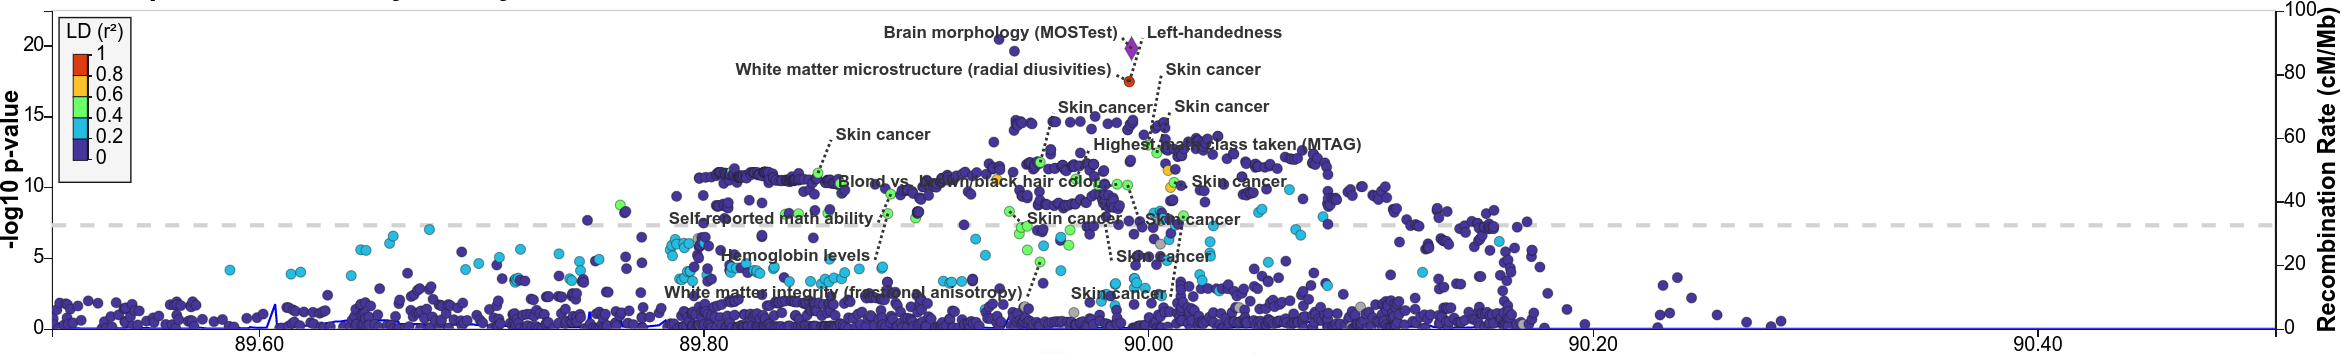
\includegraphics[width=\linewidth]{tubb3.png}
		}
		\par\medskip
		\subfloat{
			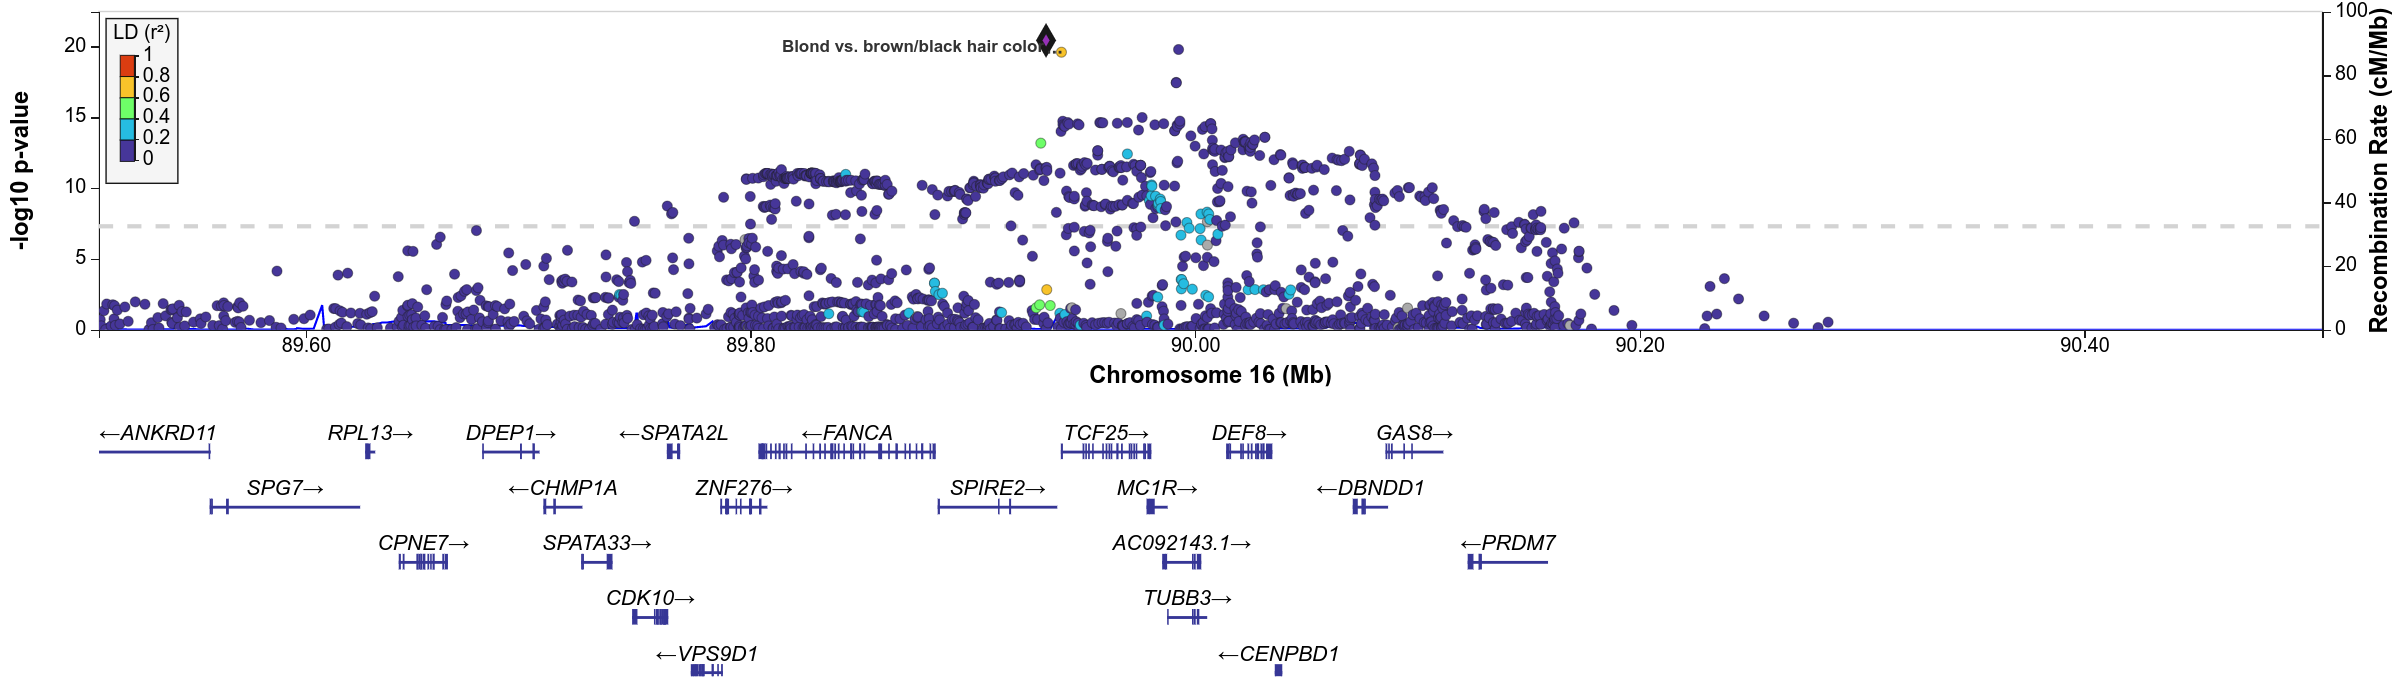
\includegraphics[width=\linewidth]{spire2.png}
		}
	\end{adjustwidth}
		\caption[Entire hemisphere \ac{gwas} Manhattan plot chromosome 16 peaks  in detail]{Scores from the entire hemisphere \ac{gwas} for chromosome 16 TUBB3 and SPIRE2 lead \acp{snp} neighborhood. -log10P values, corresponding LD $r^2$ scores and cross-trait \acp{snp} annotations are shown, as retrieved by LocusZoom tool \cite{Boughton2021}. With a purple rhombus shape the point corresponding to the reference \ac{snp} for LD computation is displayed, rs111398992 (TUBB3) and rs72813426 (SPIRE2) on the top and middle graph respectively. At the bottom, a genes mapping, based on the GRCh37 build, is displayed for that region.}
		\label{fig:chr16}
\end{figure}


\section{Contributions}
In the current study, a detailed  data-driven multi-level analysis statistically elucidated the origins of cortical asymmetry, a complex multivariate phenotypic trait, on healthy individuals of European origin from the largest known \ac{mri} database to date, UK Biobank \cite{Littlejohns2020}. The degree to which plasticity effect is dispersed throughout the brain was statistically mapped using 2-way \ac{anova} and genetically quantified, through heritability studies. A coarse-to-fine data-driven segmentation identified homogeneously symmetric regions, without any prior anatomic knowledge.  Novel causal region-specific genetic variants were identified after \ac{mvgwas} on the derived partitions, complementing the existing literature \cite{Sha2021}. Different spatially-dependent genetic profiles were identified. Connections with biological pathways, concerning intra- and extra-cellular organization and the formation of symmetry axes, were made, by examining protein-protein interactions. The effect of a strong regulating, spatially dependent epigenetic effect on development was determined. Furthermore, gender-controlled epigenetic modifications appeared to affect cortical asymmetry. Gene- and \ac{snp}-level associative studies  with other genetically-driven traits led to the establishment of a tight genetic connection between  brain shape and asymmetry, while strong \ac{snp}-level genetic correlation was detected relatively to intellectual skills, handedness, \ac{ocd}, \ac{pd} and neuroticism. At the same time, computational acceleration was achieved, without observable loss in accuracy, through the application of simple operations, such as the average shape downsampling discussed in \autoref{sec:methods_on_pheno} that made the statistical analysis feasible, and the mean substitution of the \acp{snp}, that permitted a significant speed up of the \ac{cca} analysis.

\section{Limitations and possible extensions}
\subsection{Limitations}

\subsubsection{First stage}
Several limitations were detected during the conduction of this study, some of which could potentially be avoided by an extended future research. As far as the first stage of the analysis is concerned, lack of access to a test-retest dataset from UK Biobank and the disproportionate permutation spaces of 2-way \ac{anova} increased the error margin of the results, and the total variability of the data was not captured, because of the small sample size used, despite the three experimental iterations aggregation. In addition, covariates control prior to the statistical analysis could potentially provide a more consistent shape normalization and improve results quality. Furthermore, adaptive remeshing, by performing non-rigid group-wise registration, in place of the used naive method, would possibly have increased the results resolution, in exchange for greater computational demands.

\subsubsection{Second stage}
At the second stage, the absence of a signed statistic from \ac{mvgwas} did not allow to deduce whether identified \acp{snp}' presence contributes positively or negatively to cortical asymmetry, while also prohibiting the application of \ac{ldsc} during cross-trait analysis. Another step of multivariate regression, possibly in the form of \ac{cca}, using the lead \acp{snp} as covariates and the phenotype as predicted variable, could produce signed effects for each significant variant. 

Furthermore, 1000G project Phase 3 \ac{snp} filtering greatly reduced the amount of significant genes, with p-values lower than 5e-8, approximately by 82\% for the entire hemisphere \ac{gwas} (table \autoref{tab:1000g_entire_hemisphere} and \autoref{fig:1000g_entire_hemisphere}), while certain partitions lost all the \acp{snp} for at least one chromosome, whose p-value is lower than the Bonferroni threshold of 5e-8/31 (table \autoref{tab:1000g_lost_bonf_chr}). Although UK Biobank makes use of the 1000G Phase 3 project as the reference genome to perform phasing and imputation \cite{Bycroft2018}, in the current study, the high percentage of significant \ac{snp} pruning implies that non-significant \acp{snp} relationships are mostly driving the correlation studies and the LD score analysis.

It is also noteworthy to mention that the initial \ac{snp}-based filtering (cf. \autoref{sub:snpbased_filt}) has pruned away variants, which could potentially have a great impact on the studied phenotypic trait. However, studying the complementary case is difficult and highly error-prone, heavily relying on the sequencing technologies. Including rare variants and indels requires a denser genotyping, feasible through whole genome sequencing (WGS) \cite{Kierczak2022,Cirulli2020}, a technology to-be applied on UK Biobank anticipated dataset update \cite{Halldorsson2022}.


\subsection{Further extensions}
A possible extension would be to expand the gene-based meta-analysis on the entire set of identified partitions (i.e., not only on the second level ones), and develop a hierarchy-dependent \ac{gsea}, to promote cohesive results and remove false positives. Enriching the Spearman cross-trait correlation analyses with a larger amount and variety of traits' \ac{gwas} scores would, in addition, offer a better support of the identified correlations. Gender-based studies, after  the extension of \ac{mvgwas} on X chromosome, could derive, using sex as a covariate in a regression setting, the degree of variance explained by gender for each gene \cite{Rawlik2016}. Partitioned-based heritability analysis, centered at the regions of interest, could provide an answer to whether localized subpopulation structures exist. Lastly, modeling the cortical asymmetry heritability profile through epistasis analysis and even statistical shape modeling, extending existing ideas \cite{Filipe2019,Claes2014,White2020}, could make an approximate measurement of cortical plasticity in a spatially dependent manner possible, providing grounds for a personalized method of cortical structure anomaly detection and diagnosis of related diseases.









\backmatter
\bibliographystyle{abbrv}
\bibliography{references}
\end{document}